% !TEX program = tectonic
% Rapport « Congress Trading Signal · couche données » — état final, fenêtre 2014-2026.
% Tous les chiffres proviennent des tables FINAL
% (data/house/tables/{an}/06_house_{an}_FINAL.csv, data/senate/tables/{an}/06_senate_{an}_FINAL.csv),
% du rapport qualité docs/RAPPORT_QUALITE.md (python -m common.quality, offline)
% et du notebook Nettoyage_Backtest_2014_2026.ipynb (table de recherche canonique).
\documentclass[11pt,a4paper]{article}
\usepackage[T1]{fontenc}
\usepackage{lmodern}
\usepackage[utf8]{inputenc}
\usepackage[french]{babel}
\usepackage[a4paper,margin=2cm]{geometry}
\usepackage{booktabs}
\usepackage{longtable}
\usepackage{array}
\usepackage{enumitem}
\usepackage{xcolor}
\usepackage{titlesec}
\usepackage{graphicx}
\usepackage{subcaption}
\usepackage{placeins}
\usepackage{needspace}
\usepackage{hyperref}
\usepackage{underscore}
\usepackage{amssymb}
\usepackage{textcomp}
\usepackage{newunicodechar}
\usepackage{tikz}
\usetikzlibrary{shapes.geometric,arrows.meta,positioning,fit,backgrounds,calc}

% Caractères Unicode → commandes LaTeX (fontes T1 sans ces glyphes)
\newunicodechar{→}{\ensuremath{\rightarrow}}
\newunicodechar{—}{\textemdash}
\newunicodechar{–}{\textendash}
\newunicodechar{…}{\ldots}
\newunicodechar{−}{\ensuremath{-}}
\newunicodechar{·}{\textperiodcentered}
\newunicodechar{œ}{\oe}
\newunicodechar{Œ}{\OE}
\newunicodechar{≈}{\ensuremath{\approx}}
\newunicodechar{×}{\ensuremath{\times}}
\newunicodechar{≤}{\ensuremath{\leq}}
\newunicodechar{≥}{\ensuremath{\geq}}
\newunicodechar{↔}{\ensuremath{\leftrightarrow}}
\newunicodechar{★}{\ensuremath{\star}}
% Guillemets : mapper les « » littéraux vers \og/\fg de babel — rendu ET extraction corrects.
\newunicodechar{«}{\og}
\newunicodechar{»}{\fg{}}

\hypersetup{colorlinks=true,linkcolor=blue!55!black,urlcolor=blue!55!black,
  pdftitle={Congress Trading Signal — Couche données}, pdfauthor={Alice Lemaire}}

\definecolor{coreC}{RGB}{37,99,159}
\definecolor{houseC}{RGB}{30,110,90}
\definecolor{senateC}{RGB}{120,60,150}
\definecolor{dataC}{RGB}{176,110,14}
\definecolor{testC}{RGB}{150,40,40}
\definecolor{netC}{RGB}{190,55,55}
\definecolor{offC}{RGB}{40,120,60}

\newcommand{\co}[1]{\texttt{\small #1}}
\newcommand{\netflag}{\textcolor{netC}{\small$\bullet$ réseau/API}}
\newcommand{\offflag}{\textcolor{offC}{\small$\bullet$ offline}}
% Encart « dans la source » sobre (filet à gauche, sans boîte colorée)
\newcommand{\srcex}[1]{\par\smallskip\noindent{\color{black!55}\rule{2pt}{\baselineskip}}\hspace{6pt}\begin{minipage}{\dimexpr\linewidth-16pt}\small\textit{Dans la source.}\ #1\end{minipage}\par\smallskip}
% \rev : encart neutralisé — rendu en prose sobre, contenu conservé.
\newcommand{\rev}[1]{\par\smallskip #1\par\smallskip}

\titleformat{\section}{\Large\bfseries}{\thesection}{0.6em}{}
\titleformat{\subsection}{\large\bfseries}{\thesubsection}{0.6em}{}
\titlespacing{\section}{0pt}{1.3em}{0.4em}
\titlespacing{\subsection}{0pt}{0.8em}{0.25em}

\tikzset{
  step/.style={rectangle, rounded corners=2pt, draw=#1, line width=0.8pt, fill=#1!8,
               text width=3.4cm, align=center, minimum height=0.95cm, font=\small},
  file/.style={rectangle, draw=gray!55, fill=gray!7, text width=3.4cm, align=center,
               font=\scriptsize\ttfamily, minimum height=0.55cm},
  lyr/.style={rectangle, rounded corners=3pt, draw=#1, line width=1pt, fill=#1!8,
              align=center, font=\small, minimum height=1.1cm},
  arr/.style={-{Latex[length=2.4mm]}, line width=0.9pt, draw=gray!65},
}

\setlength{\parindent}{0pt}
\setlength{\parskip}{4pt}
\setlength{\emergencystretch}{3em}
\renewcommand{\arraystretch}{1.2}

\begin{document}

% ============================ EN-TÊTE COMPACT ============================
\begin{center}
{\small\itshape Document de recherche — livrable Ramify}\\[3pt]
{\Huge\bfseries Congress Trading Signal}\\[3pt]
{\Large\bfseries La couche données}\\[5pt]
{\normalsize Extraction, identification, enrichissement et validation honnête des déclarations\\
boursières du Congrès américain — Chambre \emph{et} Sénat, 2014--2026}\\[6pt]
{\large\bfseries Alice Lemaire}\quad\textperiodcentered\quad{\small\today}
\end{center}
\vspace{2pt}\hrule\vspace{6pt}

% ============================ RÉSUMÉ ============================
\section*{Résumé}
Les membres du Congrès américain déclarent leurs transactions boursières au titre du \emph{STOCK Act}.
Exploiter ces déclarations — par exemple via une stratégie de \emph{copy-trading} — suppose au préalable
une couche données propre, traçable et honnêtement validée. Ce rapport décrit cette couche, de
l'acquisition des sources jusqu'à la table de recherche finale, pour les \textbf{deux chambres} du
Congrès sur \textbf{treize ans (2014--2026)}. En bref~:
\begin{itemize}[nosep,leftmargin=1.5em]
\item \textbf{Corpus} — \textbf{170\,920} lignes brutes reconstruites depuis les sources officielles,
soit \textbf{169\,000 transactions uniques} après dédup cross-année des re-divulgations~:
\textbf{151\,989} pour la \textbf{Chambre des représentants} (58\,728 électroniques + 93\,261 OCR) et
\textbf{17\,011} pour le \textbf{Sénat} (13\,026 électroniques + 3\,985 OCR papier).
\item \textbf{Couverture} — \textbf{100\,\%} de l'univers officiel~: les \textbf{8\,252 PTR} listés par
l'index annuel du \emph{House Clerk} sont tous traités (7\,568 avec transactions, 582 manuscrits écartés
par une politique écrite et rejouable, 102 sans transaction retenue — chacun motivé).
\item \textbf{Identité} — \textbf{100\,\%} des lignes rattachées à un \co{bioguide_id} officiel
(\textbf{367} membres à la Chambre, \textbf{78} au Sénat), avec parti et commissions.
\item \textbf{Enrichissement} — ticker, secteur \textbf{GICS$\rightarrow$ETF SPDR}, type d'actif,
montant \emph{midpoint}, ancienneté~: le \textbf{contrat de 12 champs métier} sur les deux chambres.
\item \textbf{Validation externe} — \textbf{Quiver Quantitative}, vérité-terrain \textbf{jamais
réinjectée}~: dans notre fenêtre, on retrouve \textbf{93,5\,\%} (Chambre) et \textbf{92,1\,\%} (Sénat)
des trades Quiver, et l'on est un \textbf{sur-ensemble} de Quiver (\textbf{+26\,524} combinaisons cotées
qu'il n'a pas, contre 38 trous inverses). Deux sources indépendantes corroborent~:
\emph{senate-stock-watcher} (100\,\% retrouvé, 2014--2020) et un miroir \emph{house-stock-watcher}
(99,5\,\% sur 2018--2026).
\item \textbf{Reproductibilité} — golden octet-à-octet (\textbf{230} fichiers Chambre + \textbf{138}
Sénat), invariants assertés, chaque transformation reproduite depuis les colonnes figées.
\item \textbf{Livrable de recherche} — la \textbf{table canonique}
\co{data/clean/transactions_backtest_2014_2026.csv}, \textbf{134\,464 lignes × 36 colonnes}~: entonnoir
justifié A$\rightarrow$D, enrichissements \emph{point-in-time}, flags de traçabilité, invariants
garantis (\S{}\ref{sec:nettoyage}).
\end{itemize}

% ============================ 1. INTRODUCTION ============================
\section{Introduction \& contexte}
Depuis le \textbf{STOCK Act} (2012), les membres du Congrès américain doivent divulguer publiquement
leurs transactions sur titres dans un \emph{Periodic Transaction Report} (PTR), en principe sous
\textbf{45 jours}. L'intuition de recherche — documentée académiquement (Ziobrowski \emph{et al.}
2004/2011, Karadas 2019) — est que ces personnes, par leur appartenance à des commissions clés
(Finance, \emph{Armed Services}, Intelligence) ou leur exposition à l'information, produisent par leurs
déclarations un \textbf{signal potentiellement exploitable}. Une stratégie de \emph{copy-trading}
consiste à répliquer ces transactions \emph{après} leur publication (anti-\emph{look-ahead}~: on date
chaque transaction par sa date de divulgation, jamais par une date postérieure connue).

Avant toute stratégie, il faut une \textbf{couche données} irréprochable~: extraire fidèlement les
déclarations des deux chambres sur \textbf{treize ans (2014--2026)}, les rattacher à la bonne personne,
les enrichir (ticker, secteur, montant) et les valider honnêtement. C'est l'objet de ce rapport. La
stratégie et le backtest associés constituent un travail de recherche séparé, hors du périmètre traité
ici.

% ============================ 2. SOURCES ============================
\section{Sources \& acquisition}
\label{sec:sources}

Le pipeline part de \textbf{sources publiques officielles}, complétées d'un \textbf{référentiel d'élus}
et de \textbf{deux services externes} (un modèle de vision pour les scans, un agrégateur pour la
validation). On indique ici \emph{où} l'on récupère quoi~; le \emph{traitement} de chaque source est
détaillé au \S{}\ref{sec:construction}.

\begin{itemize}[leftmargin=1.4em]
\item \textbf{Chambre des représentants — \href{https://disclosures-clerk.house.gov/FinancialDisclosure}{\emph{House Clerk}}.} Source publique sans barrière~: une archive
ZIP annuelle contenant un \textbf{index XML} (\co{\{an\}FD.xml}) qui liste tous les dépôts. On retient les
PTR (\co{FilingType=P}) et on télécharge le PDF de chacun (\co{house/acquire.py} porte le téléchargement
des index et des PDF). L'index annuel fait \textbf{autorité} sur l'appartenance d'un document à son
année~: un dépôt tardif — jusqu'à trois ans après les transactions — reste rattaché à l'année de son
formulaire. La couverture est \textbf{totale}~: 100\,\% des \textbf{8\,252 PTR} de l'univers officiel
2014--2026 sont traités (\S{}\ref{sec:qualite}).
\item \textbf{Sénat — \href{https://efdsearch.senate.gov/search/home/}{\emph{eFD}}} (\emph{Electronic Financial Disclosure}). L'API de recherche du Sénat
(\co{report_types=[11]} = PTR), accessible après acceptation d'un formulaire d'accord. Chaque dépôt est
soit une \textbf{page HTML} électronique, soit une \textbf{image papier} scannée.
\item \textbf{Référentiel des élus — \href{https://github.com/unitedstates/congress-legislators}{\emph{congress-legislators}}.}\label{sec:reference} Une déclaration ne
donne qu'un \emph{nom}~; ce jeu de données ouvert fournit, pour chaque membre, son identifiant officiel
(\href{https://bioguide.congress.gov/}{\co{bioguide_id}}), son \textbf{parti} et ses \textbf{commissions} — avec un repli sur des YAML embarqués
dans le dépôt pour rester reproductible hors-ligne.
\item \textbf{Lecture des scans — \href{https://www.anthropic.com}{\emph{Claude Vision}}.}\label{sec:vision} Une part importante des déclarations de la
Chambre et tout le papier du Sénat n'existent que comme \textbf{images}. On les lit avec l'API Claude
Vision (\co{claude-sonnet-4-6}), qui \emph{lit} \textbf{et} \emph{structure} directement le formulaire en
transactions (sortie JSON stricte, cache versionné).
\item \textbf{Validation — \href{https://www.quiverquant.com/congresstrading/}{\emph{Quiver Quantitative}}.} Agrégateur commercial des transactions du Congrès,
utilisé comme \textbf{vérité-terrain externe}~: on mesure si notre extraction concorde, \textbf{sans jamais
réinjecter} ses données.
\end{itemize}

\textbf{Deux dates par déclaration.} Chaque transaction porte une \textbf{date d'opération}
(\co{transaction_date}, quand le trade a eu lieu) et une \textbf{date de divulgation} (\co{disclosure_date},
quand le dépôt devient public). Toute la chronologie s'appuie sur la divulgation — principe
\textbf{anti-\emph{look-ahead}}~: une stratégie ne peut copier un trade qu'\emph{après} sa publication,
jamais à sa date d'opération, antérieure et inconnue du marché au moment du dépôt.

% ============================ 3. ARCHITECTURE ============================
\section{Architecture \& méthodologie}
\label{sec:archi}

\subsection{Un contrat partagé et deux orchestrateurs jumeaux}
\label{sec:archi-couches}
Le code suit une \textbf{architecture symétrique}~: un \textbf{contrat universel partagé} (\co{common/},
11 modules) et \textbf{deux orchestrateurs jumeaux} (\co{house/} et \co{senate/}) qui s'appuient dessus.
\co{common/} porte ce qui est commun aux deux chambres — schéma, référentiel, OCR de référence, secteur,
ancienneté, validation, diagnostic Quiver, qualité, orchestration~; ce qui dépend de la source —
acquisition, matcher d'identité, montants, ticker, OCR de production, réconciliation Quiver — vit dans
\co{house/} et \co{senate/}. Les données et les tests complètent l'ensemble.

\begin{center}
\begin{tikzpicture}
\node[lyr=houseC, text width=6.1cm] (h) at (-3.4,1.8) {\textbf{\color{houseC}house/} \;(9 modules)\\[1pt]\footnotesize orchestrateur Chambre des représentants\\\footnotesize \co{acquire} · \co{digital} · \co{classify_scans} · \co{ocr} · \co{identity} · \co{amounts} · \co{tickers} · \co{quiver} · \co{echantillon}};
\node[lyr=senateC, text width=6.1cm] (s) at (3.4,1.8) {\textbf{\color{senateC}senate/} \;(8 modules)\\[1pt]\footnotesize orchestrateur Sénat\\\footnotesize \co{digital} · \co{ocr} · \co{ocr_engine} · \co{fusion} · \co{identity} · \co{ticker} · \co{quiver} · \co{census_probe}};
\node[lyr=coreC, text width=12.6cm] (c) at (0,-0.6) {\textbf{\color{coreC}common/} \;(11 modules) — le contrat UNIVERSEL partagé\\[1pt]\footnotesize reference · schema · sector\_enrich · vision\_ocr · crosscheck · quality · quiver\_diagnosis · quiver\_scopes · enrich\_tenure · report\_pdf · \textbf{pipeline}};
\node[lyr=dataC, text width=8.6cm] (d) at (-2.0,-2.8) {\textbf{\color{dataC}data/} — entrées \& sorties\\\footnotesize \co{\{chambre\}/tables/\{an\}/}, PDF, scans, caches~;\\\footnotesize \co{reference/} (référentiels transverses) · \co{clean/} (table de recherche)};
\node[lyr=testC, text width=3.0cm] (t) at (4.1,-2.8) {\textbf{\color{testC}tests/}\\\footnotesize filet « zéro changement »};
\draw[arr] (h) -- (c); \draw[arr] (s) -- (c);
\draw[arr] (c) -- (d); \draw[arr] (c.south) -- (t.north);
\end{tikzpicture}
\end{center}
Les deux orchestrateurs portent les \textbf{mêmes rôles} (\co{digital}, \co{ocr}, \co{identity},
\co{quiver}\dots)~; seules leurs implémentations diffèrent, là où les sources l'imposent. Les quelques
\textbf{asymétries de structure} sont assumées et toutes dictées par la source~: au Sénat, la fusion et le
moteur OCR forment leurs propres modules (\co{fusion.py}, \co{ocr_engine.py}) là où la Chambre les garde
\emph{en ligne} dans \co{house/ocr.py}~; et le calcul des montants a un module dédié côté Chambre
(\co{amounts.py}) quand le Sénat l'intègre à ses propres modules, chaque chambre gardant sa convention de
fourchette. La fusion séparée du Sénat, elle, tient au \textbf{volume}~: l'enrichissement y passe sur
\emph{tout} le corpus en une fois (\S{}\ref{sec:socr}), quand la Chambre traite année par année.

\subsection{Le flux de bout en bout}
\label{sec:pipeline}

\begin{center}
\begin{tikzpicture}[every node/.style={font=\footnotesize}, node distance=4mm]
% --- Étiquettes de bandes (bord gauche) ---
\node[font=\scriptsize\bfseries, text=gray!55, rotate=90] at (-7.9,0) {Acquisition};
\node[font=\scriptsize\bfseries, text=gray!55, rotate=90] at (-7.9,-1.9) {Tri};
\node[font=\scriptsize\bfseries, text=gray!55, rotate=90] at (-7.9,-4.5) {Extraction};
\node[font=\scriptsize\bfseries, text=gray!55, rotate=90] at (-7.9,-9.8) {Tronc commun partagé};
% --- Acquisition (2 sources) ---
\node[step=dataC, fill=dataC!10, text width=5.4cm] (acqH) at (-4.0,0)
  {\textbf{\color{houseC}Chambre des représentants}\\[1pt]\footnotesize \emph{House Clerk} → index XML → PDF};
\node[step=dataC, fill=dataC!10, text width=5.4cm] (acqS) at (4.0,0)
  {\textbf{\color{senateC}Sénat}\\[1pt]\footnotesize \emph{eFD} → liste des dépôts (HTML ou papier)};
% --- Tri / type de document : 4 formes + manuscrit gated ---
\node[step=houseC, text width=3.0cm] (hpdf) at (-6.0,-1.9) {\textbf{PDF lisible}\\\footnotesize couche texte présente};
\node[step=houseC, text width=3.0cm] (hscan) at (-2.6,-1.9) {\textbf{scan tapé}\\\footnotesize image, souvent couchée};
\node[step=senateC, text width=3.0cm] (shtml) at (2.6,-1.9) {\textbf{page HTML}\\\footnotesize déclaration eFD};
\node[step=senateC, text width=3.0cm] (sgif) at (6.0,-1.9) {\textbf{image papier}\\\footnotesize \co{.gif}, déjà droite};
\node[file, text width=2.8cm, fill=gray!12, draw=testC] (hC) at (-2.6,-3.3) {\footnotesize scan manuscrit → écarté (politique rejouable)};
% --- Extraction : une phrase de ce qui se passe ---
\node[step=houseC, text width=3.0cm] (hpar) at (-6.0,-4.3) {\textbf{parsing déterministe}\\\footnotesize chaque transaction repérée dans le texte\\[1pt]\textbf{\color{houseC}58\,728}};
\node[step=houseC, text width=3.0cm] (hvis) at (-2.6,-5.0) {\textbf{OCR Claude Vision}\\\footnotesize redressée, lue en JSON\\[1pt]\textbf{\color{houseC}93\,261}};
\node[step=senateC, text width=3.0cm] (spar) at (2.6,-4.3) {\textbf{lecture des tableaux}\\\footnotesize colonnes par appariement flou\\[1pt]\textbf{\color{senateC}13\,026}};
\node[step=senateC, text width=3.0cm] (svis) at (6.0,-4.3) {\textbf{OCR Claude Vision}\\\footnotesize image déjà droite\\[1pt]\textbf{\color{senateC}3\,985}};
% --- Convergence : la clé naturelle ---
\node[step=coreC, fill=coreC!12, text width=12.6cm] (conv) at (0,-6.9)
  {\textbf{lignes normalisées} — déclarant, \co{transaction_date}, \co{disclosure_date}, \co{asset_description}, \co{operation_type}, \co{amount_range}, \co{owner} \emph{(les 7 champs de la clé naturelle)}};
% --- Tronc commun ---
\node[step=coreC, text width=12.6cm] (ident) at (0,-8.3)
  {\textbf{identité} — le nom libre est résolu en identifiant officiel \co{bioguide_id} (+ parti, commissions) via le référentiel partagé};
\node[step=coreC, text width=12.6cm] (enr) at (0,-9.7)
  {\textbf{enrichissement} — ticker (explicite → dictionnaire → LLM → récupération) · secteur \textbf{GICS → ETF SPDR} · montant ramené à son \emph{milieu} · ancienneté};
\node[file, text width=12.6cm, fill=houseC!10, draw=coreC, line width=1pt] (fin) at (0,-11.0)
  {\textbf{TABLE FINALE} — \textbf{169\,000 uniques} (170\,920 lignes) · \co{06_\{ch\}_\{an\}_FINAL.csv} · 28 colonnes · \textbf{contrat 12 champs métier}};
\node[step=netC, fill=netC!8, text width=12.6cm] (val) at (0,-12.3)
  {\textbf{validation Quiver} — 3 niveaux de strictesse (existence / date / champs), \textbf{jamais réinjectée}};
\node[file, text width=12.6cm, fill=dataC!10, draw=dataC, line width=1pt] (clean) at (0,-13.6)
  {\textbf{TABLE DE RECHERCHE} — \textbf{134\,464 × 36} · \co{data/clean/transactions_backtest_2014_2026.csv} · entonnoir A→D + enrichissements point-in-time (\S{}\ref{sec:nettoyage})};
% --- Bandeau méta : annotation portant sur tout le pipeline (pas une étape de flux) ---
\node[draw=gray!50, dashed, rounded corners=2pt, fill=gray!6, text width=12.4cm, align=center,
      font=\scriptsize, inner sep=4pt] (meta) at (0,-14.9)
  {\textbf{Orchestré} par \co{common.pipeline} (sous-processus) · \textbf{figé} par un golden octet-à-octet · \textbf{rapport qualité} (six contrôles, lecture seule)};
% --- arrows ---
\draw[arr] (acqH) -- (hpdf); \draw[arr] (acqH) -- (hscan);
\draw[arr] (acqS) -- (shtml); \draw[arr] (acqS) -- (sgif);
\draw[arr] (hscan) -- (hC);
\draw[arr] (hpdf) -- (hpar); \draw[arr] (hscan) -- (hvis);
\draw[arr] (shtml) -- (spar); \draw[arr] (sgif) -- (svis);
\draw[arr] (hpar) |- (conv); \draw[arr] (hvis) |- (conv);
\draw[arr] (spar) |- (conv); \draw[arr] (svis) |- (conv);
\draw[arr] (conv) -- (ident); \draw[arr] (ident) -- (enr); \draw[arr] (enr) -- (fin); \draw[arr] (fin) -- (val);
\draw[arr] (val) -- (clean);
\end{tikzpicture}
\end{center}

\subsection{À quoi ressemble la donnée}
\label{sec:numbering}
La couche finale, ce sont \textbf{26 fichiers} \co{06_\{chambre\}_\{an\}_FINAL.csv} (13~ans $\times$
2~chambres), rangés sous \co{data/house/tables/\{an\}/} et \co{data/senate/tables/\{an\}/}. Chaque
\textbf{ligne} est une transaction et porte \textbf{28 colonnes} (détail en annexe~\ref{anx:schema}).
Concrètement~:

\textbf{Une transaction cotée} (Sénat). Le sénateur \co{M000355} — \emph{A.~Mitchell McConnell, Jr.},
Républicain, KY — déclare l'\textbf{achat} de \textbf{WFC} (\emph{Wells Fargo \& Company}), une action
(\co{Stock}) du secteur \textbf{Financials} mappé sur l'ETF \textbf{XLF}, pour \textbf{\$1\,001--15\,000},
détenue par le conjoint, date jugée \emph{plausible}. Tous les champs « métier » sont renseignés.

\textbf{Une transaction non cotée} (Chambre des représentants), en contraste, montre les \textbf{trous
légitimes}~: le représentant \emph{Jefferson Shreve} déclare une \emph{JP~Morgan 3-year auto callable
buffer note} — un produit structuré qui n'a \textbf{ni ticker, ni secteur, ni ETF} (ces colonnes sont
vides) parce qu'il n'est \emph{pas} coté en Bourse. Ce n'est pas un défaut d'extraction~: il n'existe pas
de symbole à lui attribuer (\S{}\ref{sec:sector}).

\textbf{Autour de ces tables}, des fichiers intermédiaires préfixés par \textbf{rôle} — \co{03_} index,
\co{05_} échecs de parsing, \co{06_} électronique, \co{06b_} OCR, \co{07*_} réconciliation Quiver — tracent
chaque étape et restent inspectables. S'y ajoutent les \textbf{référentiels transverses} de
\co{data/reference/} — renommages et délistages de tickers, carte ticker~$\rightarrow$~secteur, photos des
commissions par Congrès (\S{}\ref{sec:nettoyage}) — et la \textbf{table de recherche} \co{data/clean/} qui en
dérive.

% ============================ 4. CONSTRUCTION ============================
\section{Construction de la donnée, étape par étape}
\label{sec:construction}

Cette section déroule le \textbf{flux de bout en bout} (\S{}\ref{sec:pipeline}) dans l'ordre des dépendances~: d'abord le référentiel d'identité (préalable partagé par toutes les pistes), puis le tri des formats, l'extraction de
chaque piste (électronique \emph{et} scannée, pour les deux chambres), enfin l'enrichissement et la table
finale. Chaque étape en donne le \textbf{résultat chiffré}.

\subsection{D'abord, savoir qui a déclaré : la résolution d'identité}
\label{sec:identity}
Une déclaration n'identifie son auteur que par un \emph{nom libre}, dont la graphie varie d'un dépôt à
l'autre — « Hon.~Earl L.~Carter », « Buddy Carter », « N.~Pelosi ». Sans clé stable, un même élu serait
compté plusieurs fois et ne pourrait être rattaché ni à son parti ni à ses commissions. La résolution
d'identité ramène donc chaque nom à l'\textbf{identifiant officiel} du membre, le \co{bioguide_id} attribué
par le \emph{Biographical Directory} du Congrès (par ex.~\co{P000197} pour Nancy Pelosi)~: unique, il rend
chaque ligne rattachable, dédupliquable et joignable au référentiel des élus.

Ce référentiel est partagé par les deux chambres. \co{common/reference.py} charge les législateurs et leurs
commissions (jeu \emph{congress-legislators}, avec repli sur des YAML embarqués) et en dérive, pour chaque
\co{bioguide_id}, le parti, les commissions et un drapeau « commission clé », ainsi qu'un \textbf{index de
noms tolérant} qui enregistre plusieurs graphies par élu — nom de famille (y compris le dernier mot d'un nom
composé), prénom, second prénom et surnom officiel. Chaque chambre construit ensuite son propre
\textbf{matcher}, car les pièges diffèrent selon la source.

À la Chambre des représentants (\co{house.identity}), la résolution d'un couple (nom, prénom) suit une
cascade à trois niveaux~: un \textbf{override manuel}, réservé à un unique cas irréductible
(« Nicholas V.~Taylor », c'est-à-dire Van Taylor)~; à défaut, une \textbf{correspondance exacte} dans
l'index, après normalisation des accents, des titres (\emph{Hon.}, \emph{Dr.}) et des suffixes, et en
essayant les diminutifs usuels (\emph{William} → \emph{Bill})~; en dernier recours, un \textbf{repli sur le
nom de famille} lorsqu'il ne désigne qu'un seul élu. Au Sénat (\co{senate.identity}), où les homonymes sont
plus fréquents, la cascade ajoute une \textbf{désambiguïsation}~: à nom de famille égal, on privilégie
d'abord un siège au Sénat, puis le titulaire \emph{en exercice}, enfin une concordance de prénom ou
d'initiale. Chaque chambre ne fige qu'un seul override (Van Taylor à la Chambre, J.D.~Vance au Sénat).
L'identité résolue, \co{house/digital.py:join_identity} et \co{senate/identity.py:enrich} y joignent le
parti, les commissions et le drapeau de commission clé issus du référentiel partagé.

La résolution rattache \textbf{100\,\%} des lignes des deux chambres~: toute ligne conservée porte un
\co{bioguide_id} — \textbf{367} membres distincts à la Chambre, \textbf{78} au Sénat, sur les treize
années~; les multiples graphies d'un même élu sont ramenées à un identifiant unique, précisément ce que la
résolution garantit. Une \emph{seule} déclaration manuscrite de 2023 a été \textbf{exclue du périmètre
membres}~: celle d'une \textbf{collaboratrice de commission} non-élue (Natalia~Henriquez, \emph{House Armed
Services Committee}), identifiée en lisant le PDF source — les agents du Congrès n'ont pas de
\co{bioguide_id}.

\subsection{Ensuite, trier les formats : électronique ou scanné ?}
\label{sec:tri}
Une même déclaration peut arriver sous deux formes qui n'appellent pas le même traitement~: un
\emph{texte} directement exploitable, que l'on analyse ligne à ligne, ou une \emph{image} qu'il faut
d'abord lire par OCR. C'est ce tri qui commande toute la suite du pipeline.

À la Chambre des représentants, le format n'est pas annoncé~: il faut le déterminer. La fonction
\co{build_manifest} (\co{house/digital.py}) ouvre chaque PDF avec \co{pdfplumber} et applique un test
binaire~: la présence d'une couche de texte (\co{bool(text.strip())}). Un texte non vide classe le document comme
\emph{lisible}, un texte vide comme \emph{non lisible} — donc destiné à l'OCR —, un fichier manquant comme
\emph{absent}. Le verdict, consigné dans \co{04_download_manifest.csv}, oriente tout le reste, et sa
simplicité fait sa robustesse. Au Sénat, le tri n'a pas à être calculé~: la recherche eFD le fournit déjà,
chaque dépôt portant son type — \co{ptr} pour une déclaration HTML électronique, \co{paper} pour une image
scannée.

Ce tri d'apparence anodine est la \textbf{fourche} du pipeline~: il fixe la composition finale du corpus —
\textbf{58\,728} transactions électroniques et \textbf{93\,261} issues de l'OCR à la Chambre,
\textbf{13\,026} et \textbf{3\,985} au Sénat (transactions uniques) — et dirige chaque document vers la
piste d'extraction décrite dans les sous-sections suivantes.

\subsection{La piste électronique de la Chambre (PDF lisibles)}
\label{sec:hdig}
Sur un PDF lisible du Clerk, les transactions ne se présentent pas comme un tableau régulier~: une même
opération peut s'étaler sur plusieurs lignes, son montant déborder sur la suivante, le ticker se glisser
entre parenthèses et le libellé de l'actif courir sur des lignes de continuation. Un simple découpage ligne
à ligne en raterait une bonne part~; l'extraction doit donc reconstruire chaque transaction avant de la
lire.

\co{house/digital.py:run_year} enchaîne les étapes. \co{load_ptr_index} lit l'index XML de l'année et en
tire la liste des dépôts (\co{03_ptr_index.csv}). Le cœur du travail revient à \co{parse_ptr}, en deux
temps~: il \textbf{recolle} d'abord les lignes coupées — un montant scindé et sa continuation sont
réassemblés en une seule ligne (\co{_join_split_lines}) — puis repère chaque transaction par une expression
régulière (\co{TXN_RE}) qui en fixe la signature~: un code d'opération (achat \co{P}, vente \co{S}, échange
\co{E}), deux dates et une fourchette de montant. La transaction localisée, il remonte de quelques lignes
pour rattacher la description de l'actif et le ticker, imprimés à proximité. Les millésimes anciens, dont
la mise en page diffère, sont lus par des \textbf{variantes dédiées} du parseur (\co{parse_ptr_legacy},
\co{parse_ptr_dual}), sélectionnées par année. \co{join_identity} joint ensuite l'identité et les
métadonnées du dépôt, et \co{finalize} calcule la clé naturelle, numérote les lots répétés
(\co{occurrence_index}) et déduplique (\S{}\ref{sec:table}).

Le résultat est écrit dans \co{06_house_\{an\}_transactions.csv}~; tout PDF lisible ne rendant aucune ligne
est consigné dans \co{05_parse_failures.csv} (aucun échec silencieux). Au total, la piste électronique de la
Chambre fournit \textbf{58\,728} transactions uniques~; sur les 8\,252 PTR officiels de l'index, \textbf{102}
seulement restent sans transaction retenue — vides réels (« \emph{nothing to report} »), amendements sans
lignes ou échecs consignés.

\srcex{Un PTR électronique de la Chambre se lit comme un tableau propre (cf.~annexe~\ref{anx:sources})~:
« Amazon.com, Inc. — Common Stock \textbf{(AMZN)} [ST] · Purchase · 03/16/2018 · \$1\,001--\$15\,000 ».
Le ticker est entre parenthèses, le type d'actif entre crochets — d'où le parsing déterministe.}

\subsection{La piste électronique du Sénat (HTML eFD)}
\label{sec:sdig}
Le Sénat ne publie pas de PDF mais des pages HTML (l'accès passe par l'accord eFD déjà décrit,
\S{}\ref{sec:sources}). La difficulté d'extraction tient aux tableaux eux-mêmes, dont l'intitulé et l'ordre des
colonnes varient d'une déclaration à l'autre.

La séquence est portée par \co{run_year}, qui interroge la liste des dépôts (\co{fetch_ptr_list},
\co{report_types=[11]}) puis récupère chaque déclaration (\co{fetch_report}, avec mise en cache sur disque —
un re-run ne retélécharge rien). \co{parse_electronic} lit alors les tableaux avec \co{pd.read_html}, qui
renvoie des \emph{DataFrames} bruts~; c'est \co{_find_col} qui y retrouve les bonnes colonnes par
\textbf{appariement flou} — on retient la colonne dont l'intitulé contient les bons mots-clés (« ticker »,
ou « asset » et « name ») —, seule approche robuste face à des en-têtes irréguliers. L'identité, la
résolution du ticker et la déduplication sont ensuite déléguées à \co{senate/identity.py:enrich}, qui
applique le matcher du Sénat (\S{}\ref{sec:identity}) et la même clé naturelle qu'à la Chambre. La sortie est
\co{06_senate_\{an\}_transactions.csv}.

Cette piste fournit \textbf{13\,026} transactions électroniques uniques pour le Sénat.

\srcex{Une déclaration eFD du Sénat est une page web (cf.~annexe~\ref{anx:sources})~: « \textbf{YUM} ·
Yum! Brands · Sale (Full) · \$1\,001--\$15\,000 · Joint », avec le ticker cliquable et la date de
transaction — d'où la lecture par \co{pd.read_html}.}

\subsection{La piste scannée de la Chambre (OCR Claude Vision)}
\label{sec:hocr}
L'autre part des déclarations de la Chambre n'existe que sous forme d'images. Un recensement des
\textbf{2\,424 PDF scannés} (\co{_scan_census.csv}) les répartit en trois familles~: \textbf{74} documents
tapés et droits (cluster~A), \textbf{1\,575} tapés mais dont l'image est \emph{couchée} (cluster~B, le gros
du volume) et \textbf{775} manuscrits (cluster~C). Un modèle de vision lit mal une page tournée, et plus mal
encore une date écrite à la main — deux difficultés traitées séparément.

La première est l'orientation. Plutôt que de demander l'angle au modèle — peu fiable, il répond presque
toujours « 90 » —, \co{detect_rotation} lui présente la page sous les quatre orientations
(\co{ROT_CANDIDATES = [0, 90, 180, 270]}) et lui fait \textbf{reconnaître} celle qui est droite. Ce
redressement améliore nettement la lecture~; le reliquat d'erreur tient à l'ambiguïté \emph{intrinsèque} des
dates manuscrites, non à la rotation.

L'extraction proprement dite, dans \co{house/ocr.py:run_ocr_year}, force un appel d'outil (\co{tool_use} sur
\co{record_transactions}, modèle \co{claude-sonnet-4-6}, sept tentatives avec \emph{backoff})~: le modèle
répond dans un schéma JSON strict, sans texte libre à re-parser, et chaque résultat est mis en cache,
versionné par \co{prompt_sha} — un re-run ne re-paie que les lots en erreur. Le prompt avait été durci en
amont sur un échantillon stratifié des trois clusters (\co{house/echantillon.py}), pour mesurer la qualité
avant le passage à l'échelle. Le ticker, absent des formulaires papier, est ré-associé à partir des symboles
vus en électronique, puis complété par une passe LLM. Le volume étant considérable, la fusion
électronique + OCR, l'enrichissement et la validation Quiver se font \textbf{année par année} pendant le run,
qui écrit directement \co{06_house_\{an\}_FINAL.csv}.

Le cluster~C manuscrit est écarté par une \textbf{politique écrite et rejouable}~: \textbf{582} documents
sont \emph{gated} — leurs dates manuscrites sont trop incertaines pour une stratégie datée (un essai contrôlé avec un modèle de vision plus puissant n'améliore pas la lecture des dates~: le goulot est l'écriture manuscrite, pas le modèle), et Quiver ne corrobore que
\textbf{12,9\,\%} des trades manuscrits (annexe~\ref{anx:metrics}, D.4). Les exceptions sont explicites et
constantes dans \co{house/ocr.py}~: trois déposants à forte perte corroborée (\co{FILERS_C_A_RECUPERER}) et
33 documents curés à la main (\co{DOCS_C_HERITES_2020_2026}) — \textbf{193} documents C figurent ainsi dans
les tables finales. Au total, la piste scannée fournit \textbf{93\,261} lignes uniques, très concentrées~:
Rohit Khanna en représente à lui seul \textbf{44,0\,\%}, et le trio de tête (Khanna, McCaul, Harshbarger)
\textbf{77,1\,\%} — de gros déposants qui déclarent exclusivement sur papier.

\srcex{Un scan de la Chambre est un \textbf{formulaire à cases} (cf.~annexe~\ref{anx:sources}), souvent
\emph{couché}~: une transaction = une ligne où l'on coche le type (Purchase/Sale), la date, et la
\textbf{fourchette de montant} (une colonne à cocher) — d'où le besoin de deskew puis de Vision.}

\subsection{La piste papier du Sénat — et pourquoi la fusion y est séparée}
\label{sec:socr}
Au Sénat, le papier est minoritaire — \textbf{quatorze} déposants sur treize ans — mais bien réel~: des
images \co{.gif}, cette fois \emph{droites}, qui ne demandent pas de redressement. \co{senate/ocr.py} les
lit avec le même moteur Vision (figé dans \co{senate/ocr_engine.py}) et écrit la table OCR \co{06b}. La
difficulté est ailleurs~: avec si peu de données, un dictionnaire de tickers reconstruit année par année
serait trop pauvre.

C'est ce qui motive la plus visible des \textbf{trois asymétries d'architecture} assumées
(\S{}\ref{sec:archi-couches}). Là où la Chambre, riche en volume, fusionne et enrichit \emph{pendant} chaque
année (\S{}\ref{sec:hocr}), le Sénat confie ces étapes à un module dédié, \co{senate/fusion.py}, exécuté une
fois toutes les années assemblées.
Sa fonction \co{main} procède en deux temps~: d'abord une fusion non destructrice \emph{par année}
(électronique + OCR, dédupliquée sur le couple \co{(natural_key_hash, occurrence_index)})~; puis un
enrichissement sur le \textbf{corpus complet, en une seule passe} — \co{senate/ticker.py:resolve_tickers}
puis \co{common/sector_enrich.py:enrich_sectors} sur toutes les années concaténées. Mutualiser ainsi le
dictionnaire de tickers fait qu'un symbole vu une année sert aux autres.

La piste papier fournit \textbf{3\,985} lignes uniques, concentrées~: Richard Blumenthal en représente
\textbf{38,7\,\%}. Ce papier est massivement composé d'actifs \textbf{non cotés} (obligations municipales
et \emph{corporate}, produits divers)~: c'est lui qui explique la couverture ticker et secteur plus basse du
Sénat, notamment en 2025--2026 (\S{}\ref{sec:qualite}) — un effet de composition des actifs, non d'extraction.

\srcex{Le papier du Sénat est un formulaire scanné (cf.~annexe~\ref{anx:sources})~: ex. « Microsoft,
NASDAQ/OTC · 2/17/10 », fourchette de montant en colonnes cochées — comme la Chambre OCR, mais droit et
sans symbole boursier imprimé (à ré-associer).}

\subsection{Donner un secteur à chaque ticker : GICS → ETF SPDR}
\label{sec:sector}
La stratégie visée ne réplique pas les transactions action par action, mais \textbf{secteur par secteur}, au
moyen d'ETF — des fonds cotés en Bourse qui répliquent tout un panier de titres, ici un secteur entier. Il
faut donc, pour chaque ticker déclaré, déterminer son secteur. La référence est la classification
\textbf{GICS} (\emph{Global Industry Classification Standard}), qui range chaque société cotée dans l'un de
onze secteurs~; chacun est associé un-à-un à l'ETF correspondant de la famille \emph{Select Sector SPDR}~:
\begin{center}\footnotesize
\co{Energy→XLE} · \co{Materials→XLB} · \co{Industrials→XLI} · \co{Consumer Discretionary→XLY} ·
\co{Consumer Staples→XLP} · \co{Health Care→XLV} · \co{Financials→XLF} · \co{Information Technology→XLK}
· \co{Communication Services→XLC} · \co{Utilities→XLU} · \co{Real Estate→XLRE}
\end{center}

\co{common/sector_enrich.py:enrich_sectors} résout le secteur par une cascade hybride qui \textbf{enregistre
sa source} (\co{sector_source})~: d'abord un secteur factuel via \co{yfinance}~; à défaut, un LLM
(\co{claude-sonnet-4-6}) contraint de répondre dans l'énumération GICS stricte et de poser un drapeau
\co{is_listed} — garde-fou qui interdit d'attribuer un secteur à un actif \textbf{non coté}~; enfin des
overrides manuels (les ETF de marché large comme \co{SPY} sont ainsi ramenés à \emph{aucun} secteur). La
table \co{GICS_TO_ETF} fait la dernière marche. Le ticker lui-même est résolu en trois voies essayées en
cascade~: un symbole \textbf{explicite} déjà imprimé, un \textbf{dictionnaire} reliant un nom à un symbole
vu ailleurs dans le corpus, puis un \textbf{LLM} muni d'un filtre « action » — pour ne jamais tickeriser une
obligation ou une muni. Une passe de \textbf{récupération} depuis le libellé de l'actif, validée par double
preuve et appliquée à la lecture, complète la cascade~: \textbf{2\,540} lignes d'actions y retrouvent leur
symbole.

Une précision s'impose sur le mot \textbf{couverture}~: c'est un \emph{taux de remplissage}, non un taux
d'exactitude. Les actifs non cotés — obligations, \emph{munis}, fonds privés — n'ont, par nature, ni symbole
ni secteur à recevoir~; une couverture inférieure à 100\,\% reflète donc avant tout la part d'actifs non
cotés, et non un défaut d'extraction.

Au terme de l'enrichissement, le ticker est renseigné pour \textbf{84,1\,\%} des lignes à la Chambre et
\textbf{77,9\,\%} au Sénat, le secteur pour \textbf{79,8\,\%} et \textbf{70,4\,\%} — les vides étant le
non-coté. Les montants sont ramenés au milieu de leur fourchette (\co{house/amounts.py:amount_midpoint}),
et l'ancienneté (\co{years_in_office}) couvre \textbf{99,9--100\,\%} des lignes des deux chambres —
calculée hors ligne et \emph{appendue} en dernière étape par \co{common/enrich_tenure.py}, de façon
octet-préservante.

\subsection{La table finale : le contrat « 12/12 »}
\label{sec:table}
Ce qui assemble les quatre pistes sans rien perdre tient en un module, \co{common/schema.py}, et en une
\textbf{clé naturelle} de sept champs~: \co{chamber}, \co{declarant_name}, \co{transaction_date},
\co{asset_description}, \co{operation_type}, \co{amount_range} et \co{owner}. Cette clé exclut délibérément
deux informations~: le \co{ticker}, ajouté plus tard à l'enrichissement, dont la présence la rendrait
instable~; et la \co{disclosure_date} (\S{}\ref{sec:sources}), car un dépôt initial et son amendement portent
le même trade et doivent rester \emph{une} transaction, non deux. Dédupliquer sur cette seule clé écraserait
pourtant des lots réels — un déposant peut légitimement déclarer le même titre plusieurs fois dans un même
dépôt, via plusieurs comptes. Pour les préserver, \co{add_occurrence_index} numérote ces répétitions
\emph{au sein d'un dépôt} (\co{occurrence_index}), et \co{dedup_canonical} ne supprime alors que les vrais
doublons d'un dépôt à l'autre~: la déduplication est \textbf{non destructrice}, opérée sur le couple
\co{(natural_key_hash, occurrence_index)}. La même clé porte la \textbf{dédup cross-année}~: une
transaction re-divulguée une autre année (amendement, rapport annuel) ne compte qu'une fois — 1\,920
re-divulgations sur 170\,920 lignes, d'où les \textbf{169\,000} transactions uniques.

La table finale compte \textbf{28 colonnes} — vingt-sept d'assemblage, plus \co{years_in_office} appendue en
dernier. Les \textbf{douze champs « métier »} exigés sont exactement la constante \co{schema.CORE_FIELDS}~:
\begin{center}\small
\co{declarant_name} · \co{chamber} · \co{party} · \co{committee_membership} · \co{transaction_date} ·
\co{disclosure_date} · \co{ticker} · \co{sector_gics} · \co{etf_proxy} · \co{operation_type} ·
\co{amount_midpoint} · \co{asset_type}
\end{center}

Reste une nuance d'honnêteté~: « présents » n'est pas « sans valeurs manquantes ». Les douze champs figurent
au schéma des deux chambres, mais trois ont des trous \textbf{légitimes}, par nature et non par défaut
d'extraction~: \co{ticker}, \co{sector_gics} et \co{etf_proxy} sont vides pour les actifs non cotés, et
\co{committee_membership} y est un instantané courant, non l'historique daté — la version
\emph{point-in-time} est portée par la table de recherche (\S{}\ref{sec:nettoyage}). Les champs toujours
renseignables — nom, chambre, parti, dates, opération, montant — sont, eux, quasi complets~; les taux de
remplissage exacts (par champ et par sous-corpus) figurent en annexe~\ref{anx:metrics}.

% ============================ 5. QUALITÉ ============================
\section{Le rapport de qualité}
\label{sec:qualite}

Une table « pleine » n'est pas pour autant une table \emph{saine}~: ses dates peuvent être incohérentes,
les délais légaux non respectés, son activité concentrée sur quelques déposants. \co{common/quality.py}
(\co{build_report}) y répond en \textbf{lecture seule} des tables finales, sans aucun appel d'API
(matplotlib en mode \co{Agg})~: il en tire la couverture de l'univers officiel, \textbf{six contrôles}, une
décomposition par \textbf{sous-corpus} et les figures regroupées en fin de section
(figure~\ref{fig:qualite}). \textbf{Sauf mention contraire, tout porte sur l'ensemble des 169\,000
transactions finales uniques — électronique et OCR confondus, les deux chambres, 2014--2026.}

\subsection{La couverture de l'univers officiel}
\label{sec:couverture}
L'index annuel du \emph{House Clerk} liste \emph{tous} les dépôts d'une année et fait \textbf{autorité} sur
l'appartenance d'un document à son année (un dépôt tardif reste rattaché à son formulaire). \textbf{100\,\%
des 8\,252 PTR officiels 2014--2026 sont traités} — parsés, OCRisés, ou écartés par une règle écrite~:

\begin{center}\small
\begin{tabular}{l rrrrr}
\toprule
\bfseries Année & \bfseries PTR officiels & \bfseries avec transactions & \bfseries gated manuscrit & \bfseries sans txn retenue & \bfseries couverts \%\\
\midrule
2014 & 708 & 613 & 94 & 1 & 100,0 \\
2015 & 728 & 627 & 97 & 4 & 100,0 \\
2016 & 765 & 651 & 110 & 4 & 100,0 \\
2017 & 801 & 708 & 82 & 11 & 100,0 \\
2018 & 830 & 752 & 68 & 10 & 100,0 \\
2019 & 683 & 616 & 52 & 15 & 100,0 \\
2020 & 733 & 688 & 35 & 10 & 100,0 \\
2021 & 680 & 653 & 15 & 12 & 100,0 \\
2022 & 624 & 602 & 14 & 8 & 100,0 \\
2023 & 460 & 447 & 2 & 11 & 100,0 \\
2024 & 451 & 440 & 5 & 6 & 100,0 \\
2025 & 515 & 503 & 6 & 6 & 100,0 \\
2026 & 274 & 268 & 2 & 4 & 100,0 \\
\midrule
\bfseries Total & \bfseries 8\,252 & \bfseries 7\,568 & \bfseries 582 & \bfseries 102 & \bfseries 100,0 \\
\bottomrule
\end{tabular}
\end{center}
{\footnotesize \emph{PTR officiels} = \co{FilingType='P'} de l'index du Clerk · \emph{avec transactions} =
documents présents dans le FINAL de l'année · \emph{gated manuscrit} = cluster C hors exceptions (politique
rejouable, \S{}\ref{sec:hocr}) · \emph{sans txn retenue} = vides réels (« \emph{nothing to report} »),
amendements sans lignes ou échecs consignés (\co{05_parse_failures}). Sénat~: pas d'index public
re-vérifiable sans re-scraper eFD~; le census interne fait foi (25 dépôts sans transaction, tous motivés
dans \co{06d_docs_sans_transaction.csv}).}

\subsection{Les six contrôles}
\begin{itemize}[nosep,leftmargin=1.5em]
\item \textbf{(a) Cohérence des dates}~: \textbf{98,1\,\%} des dates de la Chambre sont exploitables
(99,8\,\% au Sénat)~; parmi elles, \textbf{99,9\,\%} respectent \co{disclosure ≥ transaction}
(99,7\,\% au Sénat). Une relecture ciblée de 12 PDF sources montre qu'environ la moitié des rares
anomalies sont des coquilles du \emph{déposant} lui-même (un PTR imprime littéralement \co{01/35/22}),
transcrites fidèlement~: aucune date n'est fabriquée, les illisibles restent flaguées.
\item \textbf{(b) Délai légal}~: \textbf{87,3\,\%} (Chambre) et \textbf{86,9\,\%} (Sénat) des dépôts dans
les 45~jours prévus par le STOCK Act~; délai médian \textbf{27~jours} (Chambre) et \textbf{24} (Sénat).
\item \textbf{(c) Distribution des montants}~: \textbf{99,4\,\%} renseignés (167\,989 lignes)~; médiane
\textbf{8\,000\,\$}, quartile supérieur \textbf{32\,500\,\$}, moyenne 58\,314\,\$, maximum 75\,M\$.
\item \textbf{(d) Couverture par membre}~: \textbf{445} déposants distincts, dont \textbf{294} ayant
déclaré au moins dix transactions et \textbf{236} actifs sur au moins trois années.
\item \textbf{(e) Devenir des achats à +12 mois}~: \textbf{67,7\,\%} des achats observables de la Chambre
sont revendus (même membre, même ticker) dans les 12 mois suivant la divulgation, \textbf{48,3\,\%} au
Sénat~; le solde serait clos d'office par une stratégie à horizon fixe.
\item \textbf{(f) Validation externe contre Quiver} — développée à la section suivante
(\S{}\ref{sec:quiver}).
\end{itemize}
Le détail par an et par champ figure dans \co{docs/RAPPORT_QUALITE.md}~; l'essentiel en
annexe~\ref{anx:metrics}.

\subsection{Les quatre sous-corpus}
Le bilan global masque des écarts marqués entre les \textbf{quatre sous-corpus} — Chambre et Sénat, chacun
en électronique et en OCR papier. D'abord, la \textbf{couverture suit la composition d'actifs}, pas la voie
d'acquisition~: la part de ticker renseigné, voisine de 84\,\% sur trois sous-corpus, tombe à
\textbf{57,4\,\%} au Sénat OCR — qui ne compte que \textbf{40\,\%} d'actions, le reste étant du non-coté
(41\,\% « autre », munis, obligations) ou du non identifié~; sur un tel corpus, Quiver — restreint aux
actions et qui ne référence guère ces déposants-papier — n'offre aucun appui (\S{}\ref{sec:quiver}). Cette
composition fait aussi baisser la couverture du Sénat en 2025--26 (montée des obligations municipales), sans
dégradation de l'extraction. Ensuite, la \textbf{concentration} du volume est extrême et croît avec le
papier~: l'indice de Gini — \textbf{0} si tous les déposants pèsent autant, \textbf{1} si un seul concentre
tout le volume — va de \textbf{0,753} (Sénat OCR — 14 déposants seulement, top-10 = 100\,\% du volume) à \textbf{0,953} pour l'OCR de la Chambre~; à la Chambre, la concentration croît nettement avec le papier (0,873 → 0,953), dont
les dix premiers déposants captent \textbf{94,7\,\%} du volume. La fiabilité des dates de l'OCR, enfin, est
suivie à part par \co{date_confidence}~: une date est jugée \emph{plausible} si le délai
dépôt$-$transaction tombe dans une fenêtre de \textbf{75~jours}~; \textbf{99,6\,\%} des lignes OCR des scans
tapés droits le sont, \textbf{96,4\,\%} des tapés tournés, \textbf{98,6\,\%} du manuscrit conservé (détail
par cluster en annexe~\ref{anx:metrics}, D.4). Le tableau résume les quatre familles~; le détail
(couverture, qualité, mix, concentration) est en annexe~\ref{anx:metrics} (D.2--D.5).

\begin{center}\small
\begin{tabular}{l r rr r rr}
\toprule
\bfseries Sous-corpus & \bfseries n & \bfseries ticker\,\% & \bfseries sect.\,\% & \bfseries médiane\,\$ & \bfseries Gini & \bfseries top-10\,\%\\
\midrule
{\color{houseC}Chambre électronique} & 58\,728 & 83,8 & 77,7 & 8\,000 & 0,873 & 57,6 \\
{\color{houseC}Chambre OCR} & 93\,261 & 84,3 & 81,1 & 8\,000 & 0,953 & 94,7 \\
{\color{senateC}Sénat électronique} & 13\,026 & 84,1 & 77,8 & 8\,000 & 0,826 & 79,5 \\
{\color{senateC}Sénat OCR} & 3\,985 & 57,4 & 46,2 & 32\,500 & 0,753 & 100,0 \\
\bottomrule
\end{tabular}
\end{center}
{\footnotesize \emph{Gini} et \emph{top-10\,\%} mesurent la \textbf{concentration} du volume entre
déposants~: le Gini va de 0 (tous pèsent autant) à 1 (un seul capte tout)~; \emph{top-10\,\%} = part du
volume détenue par les dix plus gros déposants du corpus. Couverture, qualité, mix et concentration par
corpus en annexe~\ref{anx:metrics} (D.2--D.5).}

\begin{figure}[p]\centering
\begin{subfigure}[t]{0.46\textwidth}\centering
  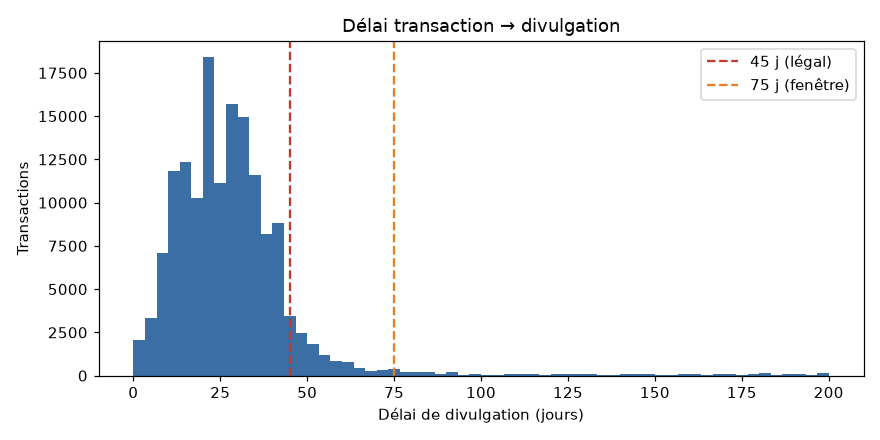
\includegraphics[width=\linewidth]{quality/delai_divulgation.png}
  \caption{Délai \co{disclosure − transaction} (0--200~j).}
\end{subfigure}\hfill
\begin{subfigure}[t]{0.46\textwidth}\centering
  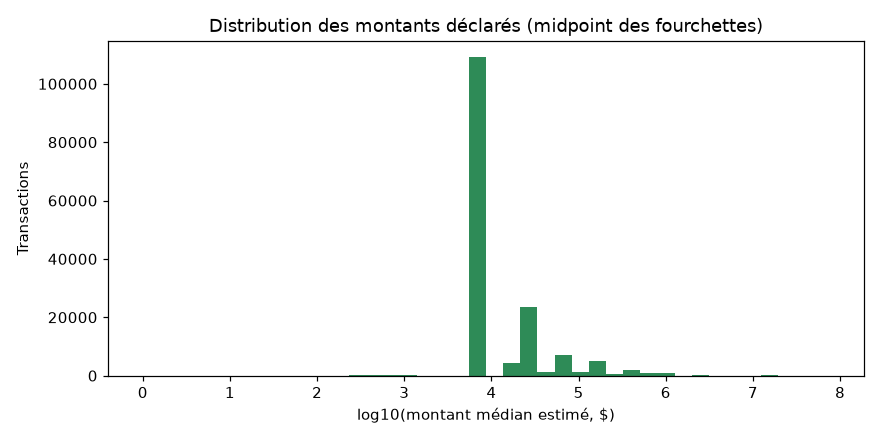
\includegraphics[width=\linewidth]{quality/distribution_montants.png}
  \caption{Distribution des montants (\co{log10}).}
\end{subfigure}

\vspace{0.5em}
\begin{subfigure}[t]{0.46\textwidth}\centering
  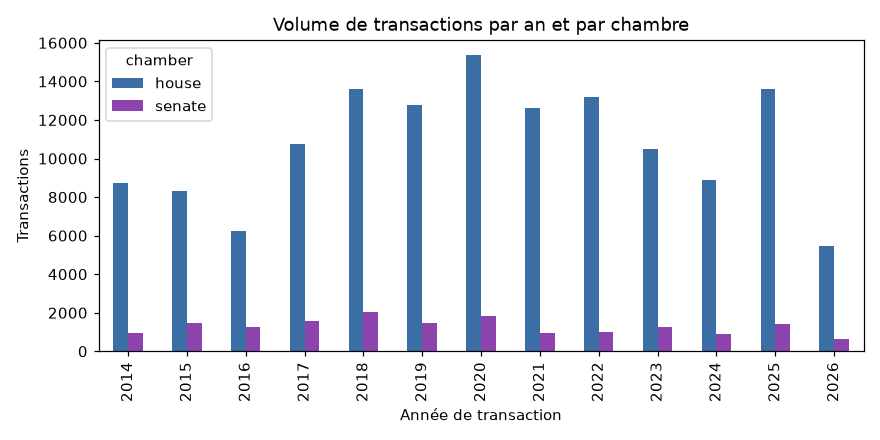
\includegraphics[width=\linewidth]{quality/transactions_par_an.png}
  \caption{Transactions par année et par chambre.}
\end{subfigure}\hfill
\begin{subfigure}[t]{0.46\textwidth}\centering
  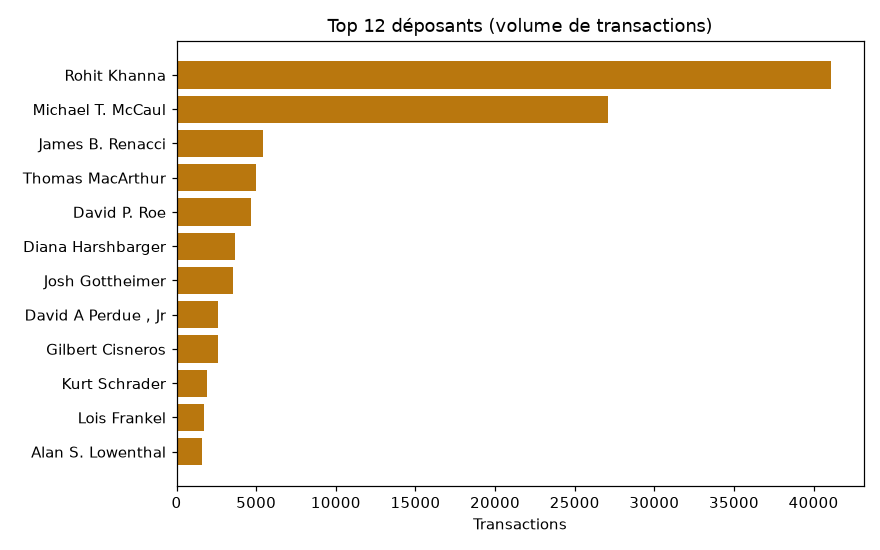
\includegraphics[width=\linewidth]{quality/top_deposants.png}
  \caption{Top~12 déposants (nombre de transactions).}
\end{subfigure}

\vspace{0.5em}
\begin{subfigure}[t]{0.46\textwidth}\centering
  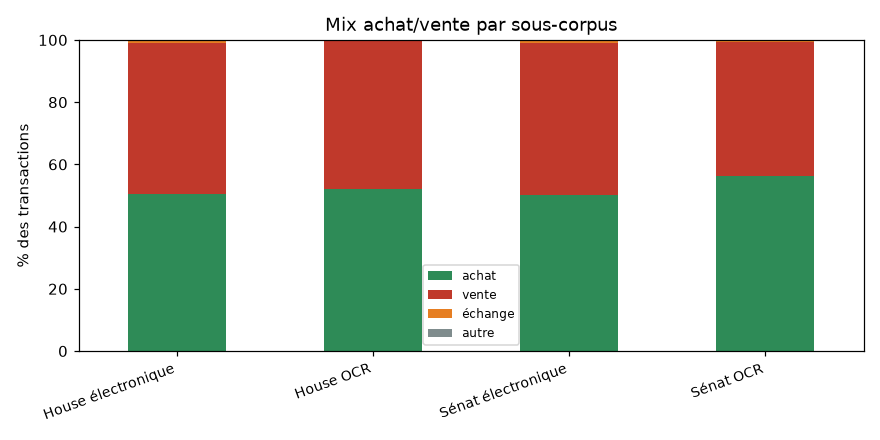
\includegraphics[width=\linewidth]{quality/mix_operations_par_corpus.png}
  \caption{Sens des opérations, \emph{par sous-corpus}.}
\end{subfigure}\hfill
\begin{subfigure}[t]{0.46\textwidth}\centering
  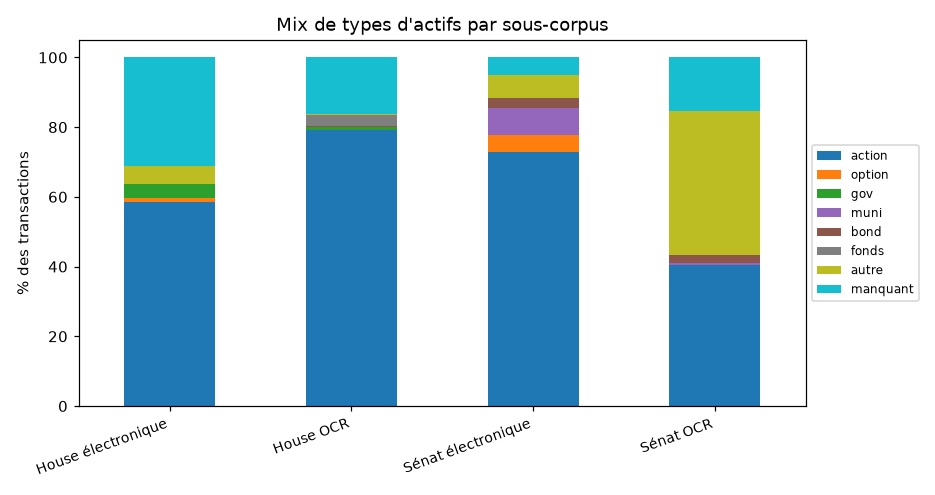
\includegraphics[width=\linewidth]{quality/mix_actifs_par_corpus.png}
  \caption{Mix de types d'actifs, \emph{par sous-corpus}.}
\end{subfigure}

\vspace{0.5em}
\begin{subfigure}[t]{0.46\textwidth}\centering
  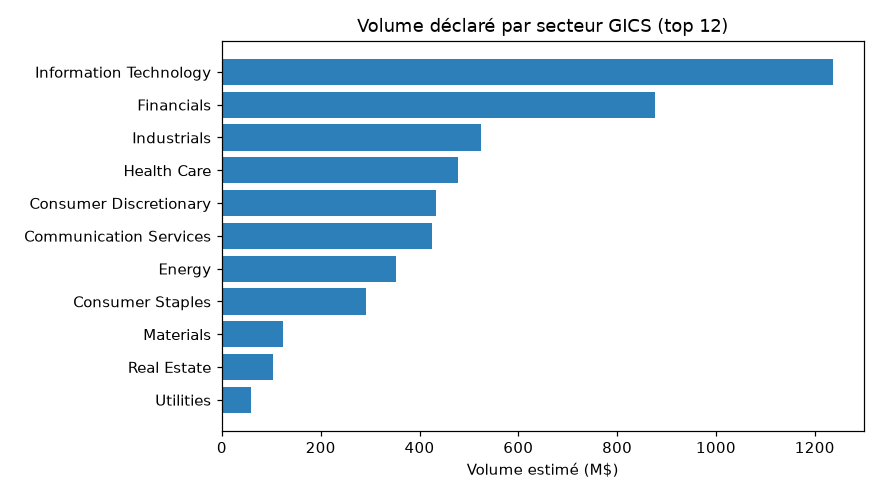
\includegraphics[width=\linewidth]{quality/volume_par_secteur.png}
  \caption{Volume par secteur GICS (top 12, ensemble).}
\end{subfigure}\hfill
\begin{subfigure}[t]{0.40\textwidth}\centering
  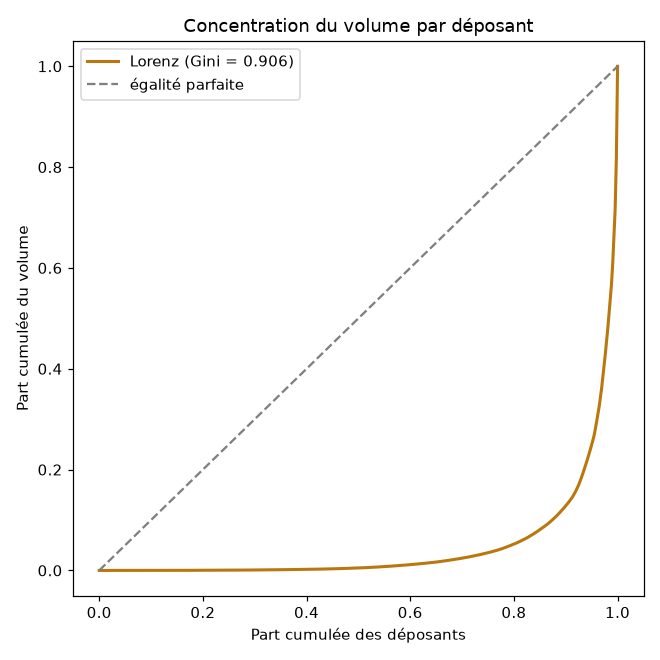
\includegraphics[width=\linewidth]{quality/concentration_lorenz.png}
  \caption{Concentration du volume (Lorenz, Gini~; ensemble).}
\end{subfigure}
\caption{\textbf{Le rapport de qualité en images}, généré par \co{common/quality.py} (lecture seule, aucun
appel API). \textbf{(a)--(d)~vues d'ensemble} sur les 169\,000 transactions finales uniques (électronique et
OCR confondus, les deux chambres, 2014--2026~; seule (c) est ventilée par chambre). \textbf{(e)--(h)~
décomposition}~: (e, f) ventilées par sous-corpus~; (g) volume par secteur et (h) concentration du volume,
sur l'ensemble.}
\label{fig:qualite}
\end{figure}

\FloatBarrier

% ============================ 6. QUIVER ============================
\section{La validation externe (Quiver)}
\label{sec:quiver}

Vérifier la justesse \emph{et la complétude} de l'extraction suppose une source indépendante. On confronte
donc le corpus final à Quiver (agrégateur commercial des mêmes déclarations) — \textbf{sans jamais le
réinjecter} — par une clé normalisée \co{bioguide × ticker × sens}, en \textbf{trois niveaux de strictesse
croissante} (\co{common/quiver_diagnosis.py}, run offline déterministe)~: \emph{a-t-on le trade~?} (sans la
date), \emph{le même trade à la même date~?} (appariement 1-à-1), \emph{que reste-t-il à corriger~?} Une
limite commande toute la lecture~: \textbf{Quiver ne suit que les actions cotées} — les lignes non cotées
(obligations, \emph{munis}, fonds privés) sont hors de son périmètre, ni validables ni en faute.

\textbf{Niveau 1 — l'existence.} Dans notre fenêtre, on retrouve \textbf{93,5\,\%} (Chambre) et
\textbf{92,1\,\%} (Sénat) des combinaisons (membre, action, sens) de Quiver~; le résidu se décompose, et le
vrai trou coté est minuscule~:
\begin{center}\footnotesize
\begin{tabular}{l rrr rrrr}
\toprule
& \bfseries Quiver (fenêtre) & \bfseries retrouvés & \bfseries incl.\,\% & \bfseries résidu & \bfseries récup. OCR & \bfseries hors périm. & \bfseries trou coté\\
\midrule
Chambre & 26\,175 & 24\,471 & \textbf{93,5} & 1\,704 & 1\,578 & 95 & 31 \\
Sénat & 4\,540 & 4\,180 & \textbf{92,1} & 360 & 7 & 353 & 0 \\
\bottomrule
\end{tabular}
\end{center}
{\footnotesize \emph{récup. OCR} = trade capté en OCR mais ticker non résolu (nom lisible)~;
\emph{hors périm.} = « ticker » Quiver non coté (CUSIP, fragment), ticker d'échange combiné, ou membre de
l'autre chambre~; \emph{trou coté} = manque au niveau \textbf{combinaison} (membre, ticker, sens — sans la date). La mesure complémentaire au \textbf{trade daté} (niveau~2) confirme \textbf{27} trous Chambre et \textbf{11} au Sénat~: ces derniers sont des occurrences datées manquantes \emph{à l'intérieur} de combinaisons par ailleurs retrouvées — les deux comptes ne s'emboîtent pas, et 27+11 = les 38 trous inverses du résumé.}

\textbf{On est un sur-ensemble de Quiver.} En sens inverse, on possède \textbf{23\,562} (Chambre) et
\textbf{2\,962} (Sénat) actions cotées que Quiver n'a pas — \textbf{+26\,524} combinaisons cotées, contre
38 trous inverses. L'électronique, lui, est quasi exact des deux côtés (98--99\,\% de concordance).

\textbf{Niveau 2 — la date.} L'appariement \textbf{1-à-1} à l'intérieur de chaque (membre, ticker, sens) —
dates identiques d'abord, puis plus proche voisin plafonné à 90~jours, quantités respectées — classe chaque
trade~:
\begin{center}\small
\begin{tabular}{l rrrrr}
\toprule
& \bfseries apparié exact & \bfseries proche (≤10\,j) & \bfseries candidats & \bfseries nous-seul & \bfseries quiver-seul\\
\midrule
Chambre & 70\,265 & 845 & 2\,202 & 39\,207 & 9\,899 \\
Sénat & 8\,766 & 0 & 0 & 3\,140 & 581 \\
\bottomrule
\end{tabular}
\end{center}
{\footnotesize \emph{proche} = voisin apparié à \textbf{≤10 j} d'écart~; \emph{candidats} = voisin entre 10 et 90~jours (date divergente, appariement incertain — parmi ces 2\,202, seules les \textbf{545} paires issues de la \emph{même déclaration} des deux côtés sont d'honnêtes candidats d'erreur de date, cf. ci-dessous)~; \emph{nous-seul} = Quiver n'a pas le trade (on est plus complet)~; \emph{quiver-seul} = absent de nos clés exactes (surtout OCR papier et non-coté). Les volumes « nous-seul » ne contredisent pas le niveau 1~: c'est le niveau de strictesse qui change (trade daté \emph{vs} combinaison).}
Les seuls candidats honnêtes d'erreur de date — les paires issues de la \textbf{même déclaration} des deux
côtés — sont \textbf{545} à la Chambre et \textbf{0} au Sénat~; un petit delta peut être une convention de
date de Quiver, et le vrai contrôle des dates reste la relecture des PDF sources (\S{}\ref{sec:qualite}).

\textbf{Niveau 3 — les autres champs.} Sur les trades présents des deux côtés (membre + ticker + date),
l'accord est de \textbf{96,8\,\%} sur le sens et \textbf{94,2\,\%} sur le montant à la Chambre
(\textbf{99,9} / \textbf{99,8\,\%} au Sénat). La liste résiduelle « à revoir » tient en trois lignes —
\textbf{27 / 11} vrais trous cotés (le seul chiffre dur), 3\,378 lignes-papier absentes de nos clés exactes
et 8\,418 + 190 « autre ticker le même jour » (bornes hautes ensemblistes, listées cas par cas dans
\co{docs/quiver_validation/}, pas des taux d'erreur).

\textbf{Honnêteté par ère.} Le taux global lisse une hétérogénéité temporelle~: au niveau action (Chambre),
\textbf{87,2\,\%} de nos actions 2020--2026 sont corroborées par Quiver, contre \textbf{58,7\,\%} sur
2014--2019 (creux 2015--2016~: 16,6\,\%). L'écart ne signale pas une erreur de notre côté~: nos actions
« en plus » pré-2020 portent des tickers réels et d'époque (vérifiés), mais \textbf{Quiver est mince avant
$\approx$\,2017} et ne peut pas les corroborer. Il y a donc \emph{moins de vérité-terrain externe avant
2017} — à garder en tête pour tout usage aval. Détail par année en annexe~\ref{anx:metrics} (D.4).

\textbf{Cross-validation indépendante (hors Quiver).} Deux sources tierces complètent le contrôle~:
\emph{senate-stock-watcher} (6\,231 transactions tickérisées 2014--2020) est couvert à \textbf{100\,\%}
par notre corpus Sénat — hors représentation des échanges, que cette source éclate en deux lignes~; un
miroir \emph{house-stock-watcher} reconstruit est retrouvé à \textbf{99,5\,\%} sur 2018--2026. Le papier du
Sénat, massivement non coté et absent de Quiver, se juge à ces contrôles internes et croisés, pas à Quiver.

% ============================ 7. NETTOYAGE BACKTEST ============================
\section{Du corpus à la table de recherche (nettoyage backtest)}
\label{sec:nettoyage}

Le corpus final décrit jusqu'ici est \emph{fidèle aux déclarations}~: il contient aussi des actifs sans
prix de marché, des dates illisibles et des opérations sans sens directionnel. Un backtest, lui, exige un
\textbf{prix}, un \textbf{sens} et un \textbf{montant}. Une étape dédiée dérive donc la \textbf{table de
recherche canonique} — \co{data/clean/transactions_backtest_2014_2026.csv}, \textbf{134\,464 lignes × 36
colonnes} — produite par le notebook \co{Nettoyage_Backtest_2014_2026.ipynb}~: exécutable hors-ligne, sans
logique dupliquée (il réutilise \co{load_final}, \co{canonical_ticker} et les référentiels transverses).

\textbf{Philosophie~: on ne retire que l'avéré inutilisable pour un backtest actions/ETF~; tout le reste
est gardé et flagué} — le doute se tranche en aval, jamais en silence.

\subsection{L'entonnoir A→D}
\begin{center}\small
\begin{tabular}{c p{9.2cm} r r}
\toprule
\bfseries Étape & \bfseries Règle exacte & \bfseries Retirées & \bfseries Restantes\\
\midrule
— & départ~: le corpus unique (\co{load_final}) & — & 169\,000 \\
A & \textbf{dates présentes \& cohérentes}~: les deux dates lisibles, divulgation $\geq$ transaction,
    année de transaction plausible ($\geq$ 2012 et $\leq$ année de dépôt) & 3\,252 & 165\,748 \\
B & \textbf{actions + ETF cotés}, « ticker d'abord »~: symbole normalisé non vide, réellement coté
    (ni CUSIP, ni préférentielle \co{\$}, ni fragment OCR), famille d'actif
    $\notin$ \{obligation, muni, gouvernement, option, autre\} & 29\,771 & 135\,977 \\
C & \textbf{direction exploitable}~: achat ou vente (les échanges, à l'économie ambiguë, sortent) & 826 & 135\,151 \\
D & \textbf{montant présent}~: \co{amount_midpoint} numérique & 687 & 134\,464 \\
\bottomrule
\end{tabular}
\end{center}
{\footnotesize 169\,000 $\rightarrow$ 134\,464 = \textbf{79,6\,\%} du corpus conservé. Chaque retrait est
motivé par l'impossibilité \emph{matérielle} de backtester la ligne, jamais par un simple champ vide
récupérable.}

\textbf{Pourquoi les lignes de l'étape B partent} — ventilation prouvée par une cellule de contrôle
(une seule cause par ligne)~:
\begin{itemize}[nosep,leftmargin=1.5em]
\item \textbf{27\,006} sans aucun ticker~: actifs non cotés (munis, obligations, sociétés privées) qui
n'ont légitimement pas de symbole — donc pas de prix~;
\item \textbf{164} tickers malformés~: préférentielles \co{\$}, deux symboles collés, fragments OCR,
CUSIP~;
\item \textbf{2\,601} options / obligations~: famille explicitement non cotée.
\end{itemize}
Le filtre raisonne \textbf{« ticker d'abord »}~: \textbf{21\,878} vraies actions/ETF au champ
\co{asset_type} vide sont \emph{gardées} grâce à leur ticker coté (un filtre « type d'abord » les jetterait
à tort)~; contrôle d'étanchéité~: \textbf{0} ligne de famille non cotée ne fuit parmi les gardées.

\subsection{Montants : une convention unique}
\begin{itemize}[nosep,leftmargin=1.5em]
\item \co{amount_midpoint} = \textbf{milieu exact de la fourchette} STOCK Act, (borne basse + borne
haute)/2, recalculé depuis \co{amount_range} sur tout le corpus — une seule convention~;
\item un montant exact déclaré (ex. \$584) reste tel quel~;
\item le palier ouvert « \emph{Over \$50,000,000} » est posé à son \textbf{plancher} (50\,M\$), pour ne
jamais inventer de masse.
\end{itemize}

\subsection{Enrichissements point-in-time et flags (aucune ligne retirée)}
Tout ce qui suit \emph{ajoute} de l'information, sans jamais filtrer~:
\begin{itemize}[nosep,leftmargin=1.5em]
\item \textbf{Parti à la date de la transaction} — depuis les \co{party_affiliations} du référentiel
officiel~: les changements de parti \emph{en cours de mandat} sont datés (Amash 2019, Mitchell 2018,
Manchin 2024)~;
\item \textbf{Commissions du Congrès de la transaction} — photos par Congrès
(\co{committees_snapshots/} sous \co{data/reference/}, Congrès 113 à 119), bascule au 3~janvier des
années impaires~;
\textbf{99,1\,\%} des lignes résolues~; \co{committees_key_flag} (fiscalité, défense, renseignement,
banque~: 54,6\,\%) — la liste complète des commissions est exportée, la recherche peut redéfinir son propre
flag sans re-générer la table~;
\item \textbf{Ticker fidèle + \co{ticker_yahoo}} — \co{ticker} reste tel que déclaré~; \co{ticker_yahoo}
est le symbole \textbf{canonique pour le join prix} (format Yahoo, renommages et fusions appliqués via
\co{ticker_renames.csv})~: \textbf{2\,817} lignes re-symbolisées, \textbf{3\,542} lignes sur titres
délistés \emph{typés} (rachat, faillite\dots) au lieu de disparaître en silence, \textbf{505} lignes
« prudence prix » (\co{flag_price_caution}~: symbole recyclé ou jambe absorbée d'une fusion, dont
l'historique du successeur ne vaut pas avant le deal)~;
\item \textbf{Classe d'actif et secteur} — \co{asset_class} (\co{stock} 128\,974 · \co{etf_broad} 2\,022 ·
\co{etf_sector} 168 · \co{unknown} 3\,300) via la carte transverse \co{ticker_sector_map.csv}~; le secteur
GICS est renseigné pour \textbf{100\,\%} des actions et \co{etf_proxy} pour \textbf{98,8\,\%} des lignes~;
un \textbf{ETF diversifié n'a pas de secteur} (\co{etf_broad}, flagué \co{is_broad_etf}) — jamais de faux
secteur~;
\item \textbf{Flags de traçabilité} — dépôt tardif $>$45~j~: \textbf{16\,349} lignes
(\textbf{12,2\,\%})~; $>$365~j~: \textbf{3\,075} (\textbf{2,3\,\%}) — l'information reste réelle et
exploitable à sa \co{disclosure_date}, on flague, on ne retire pas~; \co{lot_size} — \textbf{11\,873}
lignes appartiennent à des \textbf{lots multi-comptes réels} (mêmes 7 champs de clé~: comptes
Self/Spouse/Joint/Child)~: \textbf{ne jamais \co{drop_duplicates()}} sur cette table.
\end{itemize}

\subsection{Les référentiels transverses (\co{data/reference/})}
\begin{itemize}[nosep,leftmargin=1.5em]
\item \co{ticker_renames.csv} — \textbf{84 entrées}~: renommages (21~: FB$\to$META, PCLN$\to$BKNG\dots),
fusions-échanges (11), rachats avec délistage (43), faillites (5), recyclages de symbole (4)~; chaque
entrée précise la \textbf{validité d'historique} du successeur (la jambe absorbée d'une fusion n'a pas de
prix avant le deal)~;
\item \co{ticker_sector_map.csv} — \textbf{4\,848 tickers} $\rightarrow$ classe d'actif, secteur GICS, ETF
proxy (4\,330 actions, 97 ETF larges, 11 ETF sectoriels, 410 non tranchés)~;
\item \co{committees_snapshots/113..119} — la composition des commissions à chaque Congrès (membres et
intitulés), source du point-in-time.
\end{itemize}

\subsection{Composition finale et garanties}
\begin{center}\small
\begin{tabular}{l rr r}
\toprule
& \bfseries 2014--2019 & \bfseries 2020--2026 & \bfseries Total\\
\midrule
{\color{houseC}Chambre des représentants} & 56\,706 & 66\,108 & \textbf{122\,814} \\
{\color{senateC}Sénat} & 7\,111 & 4\,539 & \textbf{11\,650} \\
\midrule
\bfseries Total & 63\,817 & 70\,647 & \bfseries 134\,464 \\
\bottomrule
\end{tabular}
\qquad
\begin{tabular}{l r}
\toprule
\bfseries Sens & \bfseries n\\
\midrule
achats (\co{buy}) & 68\,250 \\
ventes (\co{sell}) & 66\,214 \\
\bottomrule
\end{tabular}
\end{center}
{\footnotesize Par sous-corpus~: Chambre OCR 75\,205 · Chambre électronique 47\,609 · Sénat électronique
9\,729 · Sénat OCR 1\,921. Ères découpées sur l'année de la transaction.}

\textbf{Invariants garantis} par assertions à l'export — la table est \emph{certifiée} sur~:
\co{bioguide_id} présent · \co{ticker} présent · \co{amount_midpoint} présent · \co{direction}
$\in$ \{\co{buy}, \co{sell}\} · chronologie (\co{lag_days} $\geq$ 0) · \co{natural_key_hash} présent —
sur 100\,\% des 134\,464 lignes.

\subsection{Dictionnaire des 36 colonnes}
{\footnotesize
\begin{longtable}{r >{\ttfamily}p{4.1cm} p{10.2cm}}
\toprule
\# & \normalfont\bfseries Colonne & \bfseries Sens \\
\midrule\endhead
\multicolumn{3}{l}{\bfseries Identité du déposant}\\
1 & bioguide_id & identifiant officiel du membre (toujours rempli) \\
2 & member_name & nom tel que déposé \\
3 & party & parti \textbf{à la date de la transaction} (point-in-time, switchs gérés) \\
4 & chamber & \co{house} / \co{senate} \\
5 & state_district & état + district \\
\midrule
\multicolumn{3}{l}{\bfseries Mandat (point-in-time)}\\
6 & committee_membership & commissions \textbf{du Congrès de la transaction} (snapshots 113--119) \\
7 & committees_key_flag & commission « clé » (fiscalité / défense / renseignement / banque) \\
8 & congress & numéro du Congrès de la transaction (bascule au 3 janvier) \\
\midrule
\multicolumn{3}{l}{\bfseries Compte \& lots}\\
9 & owner & titulaire du compte (Self / Spouse / Joint / Child) \\
10 & occurrence_index & rang du lot au sein du dépôt \\
11 & lot_size & taille du lot de lignes identiques (mêmes 7 champs de clé) — \textbf{ne jamais dédupliquer} \\
\midrule
\multicolumn{3}{l}{\bfseries Titre}\\
12 & ticker & symbole \textbf{fidèle} à la déclaration \\
13 & ticker_yahoo & symbole \textbf{canonique pour le join prix} (format Yahoo, renommages appliqués) \\
14 & flag_ticker & statut de normalisation (\co{ok} / \co{classe_convertie} / \co{contient_chiffre}) \\
15 & is_delisted & titre sorti de cote (booléen) \\
16 & delist_type & type de sortie de cote (rachat, faillite, fusion-échange\dots) \\
17 & flag_price_caution & prudence au join prix (symbole recyclé, jambe absorbée d'une fusion) \\
\midrule
\multicolumn{3}{l}{\bfseries Classe \& secteur}\\
18 & asset_class & \co{stock} / \co{etf_sector} / \co{etf_broad} / \co{unknown} \\
19 & asset_type & type d'actif déclaré à la source \\
20 & is_broad_etf & ETF diversifié (sans secteur GICS, par nature) \\
21 & sector_gics & secteur GICS (actions seulement) \\
22 & etf_proxy & ETF SPDR du secteur \\
\midrule
\multicolumn{3}{l}{\bfseries Opération}\\
23 & direction & \co{buy} / \co{sell} \\
24 & amount_midpoint & \textbf{milieu exact} de la fourchette (convention unique) \\
25 & amount_range & fourchette source déclarée \\
26 & amount_range_repaired & indicateur~: borne haute de la fourchette reconstituée à la lecture \\
\midrule
\multicolumn{3}{l}{\bfseries Dates}\\
27 & transaction_date & date de la transaction \\
28 & disclosure_date & date de divulgation — \textbf{l'entrée anti-look-ahead} \\
29 & lag_days & divulgation $-$ transaction (jours) \\
30 & flag_late_filing & dépôt au-delà des 45~j légaux \\
31 & flag_very_late_filing & dépôt au-delà de 365~j \\
\midrule
\multicolumn{3}{l}{\bfseries Traçabilité}\\
32 & doc_id & identifiant du document source (PTR / eFD) \\
33 & provenance & piste d'acquisition (électronique / OCR, par chambre) \\
34 & ticker_source & origine du ticker (explicite / dictionnaire / LLM / récupéré) \\
35 & natural_key_hash & clé de déduplication (7 champs) \\
36 & asset_description & libellé source de l'actif \\
\bottomrule
\end{longtable}}

% ============================ 8. REPRODUCTIBILITÉ ============================
\section{Assurance qualité \& reproductibilité}
\label{sec:repro}

Le pipeline n'est pas rejouable hors ligne~: le \emph{scraping} exige le réseau, l'OCR une API, et rejouer
une année électronique produirait même une table vide, puisque les PDF lisibles ont été parsés puis
écartés. La correction ne peut donc se prouver par simple ré-exécution~; on l'établit, plus solidement, par
\textbf{reproduction déterministe depuis les colonnes figées}.

Quatre garde-fous s'y emploient. D'abord, un \textbf{golden octet-à-octet}~: l'empreinte SHA-256 de chacune
des sorties est figée — \textbf{230} fichiers à la Chambre, \textbf{138} au Sénat, 368 tables CSV — et
\co{check_golden.py} (respectivement \co{senate_check_golden.py}) doit afficher « ZÉRO ÉCART » à chaque
exécution. Ensuite, des \textbf{reproductions fonction par fonction}~: \co{test_senate_repro} recompose
chaque hash de clé naturelle (8\,841/8\,841 sur les années 2020--2026) et réassocie identité et ticker à
partir des seules colonnes figées~; côté Chambre, \co{test_schema}, \co{test_amounts_tickers},
\co{test_identity}, \co{test_tenure} et \co{test_crosscheck} jouent le même rôle. Troisièmement,
\co{test_vision_sha} et \co{test_incremental} vérifient que le \co{prompt_sha} est stable — un second
passage OCR ne déclenche aucun appel. Enfin, \co{audit_metrics.py} recompute l'ensemble des métriques et
\emph{asserte} les invariants porteurs (totaux, identité 100\,\%, 367/78 bioguides)~: c'est la source de
vérité chiffrée de ce rapport. Au total, \textbf{dix scripts de régression}, tous au vert.

La \textbf{table de recherche canonique se recompose exactement}~: le rapport qualité rejoue l'entonnoir
A$\rightarrow$D avec les mêmes primitives que le notebook et \emph{asserte} l'égalité (134\,464 lignes)
avec le fichier publié~; l'export du notebook vérifie ses six invariants (\S{}\ref{sec:nettoyage}). Les
réconciliations Quiver, déterministes grâce à un tri à départage stable, sont figées dans le golden au même
titre que les tables.

% ============================ 9. LIMITES ============================
\section{Limites (honnêteté)}
\label{sec:limites}
\begin{itemize}[nosep,leftmargin=1.5em]
\item \textbf{Manuscrits \emph{gated}}~: \textbf{582} documents manuscrits (cluster C) sont écartés par
une \textbf{politique écrite et rejouable} (exceptions explicites dans \co{house/ocr.py})~: leurs dates
sont trop incertaines pour une stratégie datée, et Quiver ne corrobore que 12,9\,\% des trades manuscrits.
Choix assumé et documenté, listes rejouables.
\item \textbf{\co{ticker}/\co{sector_gics}/\co{etf_proxy} structurellement absents} pour munis et
obligations~: les actifs \textbf{non cotés} n'ont ni symbole ni secteur, par nature. C'est aussi ce qui met
une partie de l'OCR (le papier du Sénat surtout) \textbf{hors périmètre Quiver}.
\item \textbf{Fourchettes STOCK Act}~: les montants déclarés sont des \emph{tranches}, pas des chiffres
exacts. \co{amount_midpoint} en prend le milieu exact (convention unique~; palier ouvert $>$50\,M\$ au
plancher)~: l'incertitude intra-tranche est irréductible.
\item \textbf{Prix des délistés — traités par type}~: via \co{ticker_renames.csv}, chaque titre sorti de
cote porte son \co{delist_type}~; au backtest, une \textbf{faillite} $\approx$ perte totale, un
\textbf{rachat} = clôture au prix du deal à sa date, une \textbf{fusion-échange} bascule sur le successeur
(historique invalide avant le deal, \co{flag_price_caution}).
\item \textbf{Commissions des tables FINAL = photo courante}~; l'historique daté (par Congrès) est porté
par la table de recherche canonique (\co{committee_membership} point-in-time, \S{}\ref{sec:nettoyage}).
\item \textbf{Vérité-terrain mince avant $\approx$\,2017}~: Quiver ne peut corroborer qu'une partie de nos
lignes pré-2017 (réelles mais peu vérifiables par lui)~; \emph{senate-stock-watcher} confirme le Sénat
2014--2020 à 100\,\%.
\item \textbf{Dates OCR résiduellement imprécises}~: quelques dates de transaction lues sur scan restent
douteuses (flaguées \co{date_confidence})~; tout usage aval entre sur \co{disclosure_date} —
l'anti-\emph{look-ahead} n'en dépend pas.
\item \textbf{Cutoffs de collecte}~: Chambre 2026-07-03, Sénat 2026-06-25 — les dépôts postérieurs ne
figurent pas dans le corpus.
\end{itemize}

% ============================ 10. PÉRIMÈTRE ============================
\section{Périmètre \& suite}
La \textbf{couche données} décrite ici est livrée~: \textbf{169\,000} transactions uniques (170\,920
lignes brutes) extraites, identifiées, enrichies (contrat 12/12), validées et reproductibles — et la
\textbf{table de recherche canonique} (\textbf{134\,464 × 36}) prête pour le backtest. La \textbf{stratégie
et le backtest} associés (copy-trading actions puis ETF sectoriels) constituent un travail de recherche
séparé, hors-périmètre de ce rapport.

% ============================ 11. CONCLUSION ============================
\section{Conclusion}
Sur deux chambres et \textbf{treize ans}, le pipeline reconstruit \textbf{170\,920} lignes
(\textbf{169\,000} transactions uniques) à partir des sources officielles, en traitant honnêtement les deux
pistes (électronique déterministe \emph{et} scannée par OCR Vision), et couvre \textbf{100\,\%} de
l'univers officiel du Clerk (8\,252 PTR). Chaque ligne est identifiée (100\,\%, 367/78 bioguides), enrichie
(contrat 12/12 sur les deux chambres) et validée contre Quiver sans jamais le réinjecter~: \textbf{93,5\,\%}
(Chambre) et \textbf{92,1\,\%} (Sénat) des trades Quiver retrouvés dans la fenêtre, un \textbf{sur-ensemble}
de Quiver (+26\,524 combinaisons cotées), corroboré par deux sources indépendantes. La correction est figée
(golden octet-à-octet, 230/138) et reproductible. Le livrable de recherche est la \textbf{table canonique
134\,464 × 36}~: entonnoir justifié, montants à convention unique, parti et commissions
\emph{point-in-time}, tickers prêts pour le join prix, délistés typés — et chaque limite connue (manuscrits
gated, non-coté, fourchettes, corroboration mince pré-2017) documentée et flaguée, jamais masquée. C'est une
couche données sur laquelle une stratégie peut être bâtie \emph{en connaissant ses limites}.

% ============================ ANNEXES ============================
\clearpage
\section{Annexes}

\subsection{Annexe A — aperçu des sources}
\label{anx:sources}
À quoi ressemble la matière première des \textbf{quatre pistes} (deux chambres × électronique/OCR).
Captures des plateformes publiques (\emph{House Clerk}, Sénat \emph{eFD}) et rendu d'un scan du dépôt.

\begin{center}
\begin{minipage}[t]{0.47\textwidth}\centering
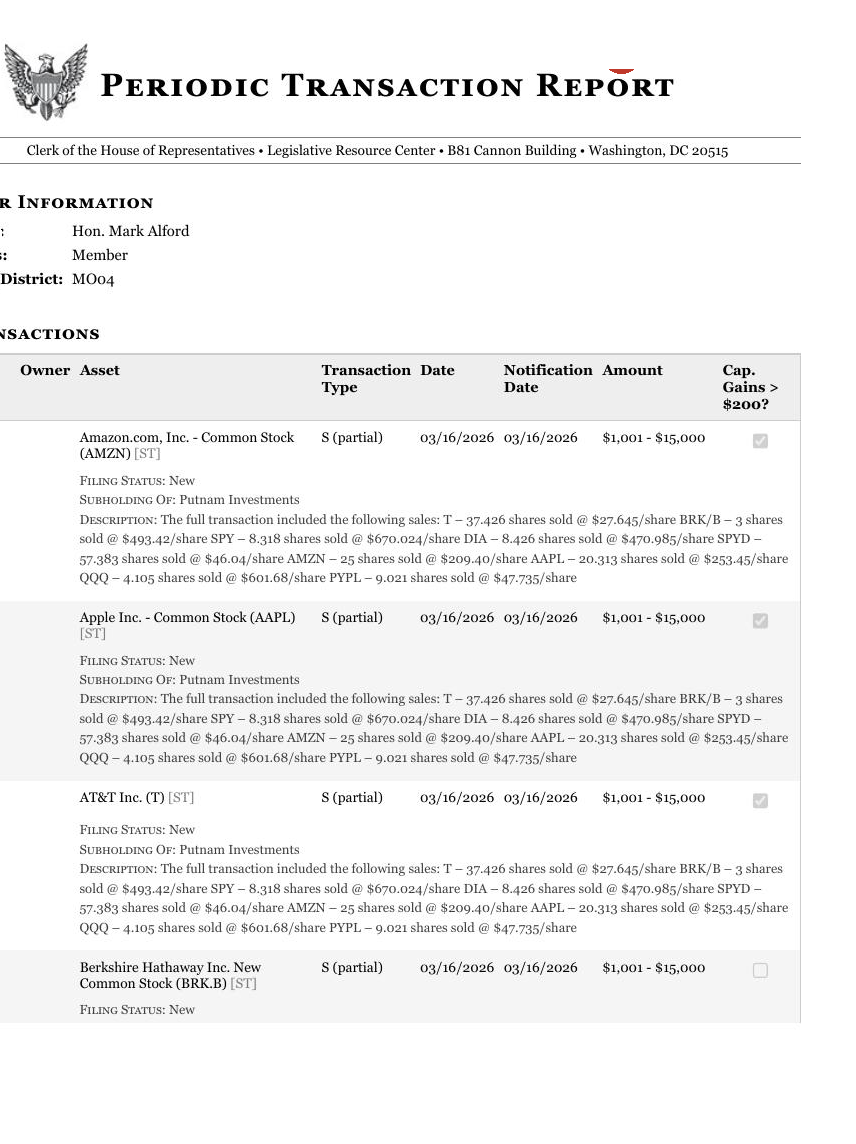
\includegraphics[height=7cm]{sources/house_digital.png}\\[3pt]
{\footnotesize\textbf{(a) Chambre — électronique.} PTR (\emph{House Clerk})~: tableau texte, ticker entre
parenthèses (AMZN), type d'actif entre crochets.}
\end{minipage}\hfill
\begin{minipage}[t]{0.47\textwidth}\centering
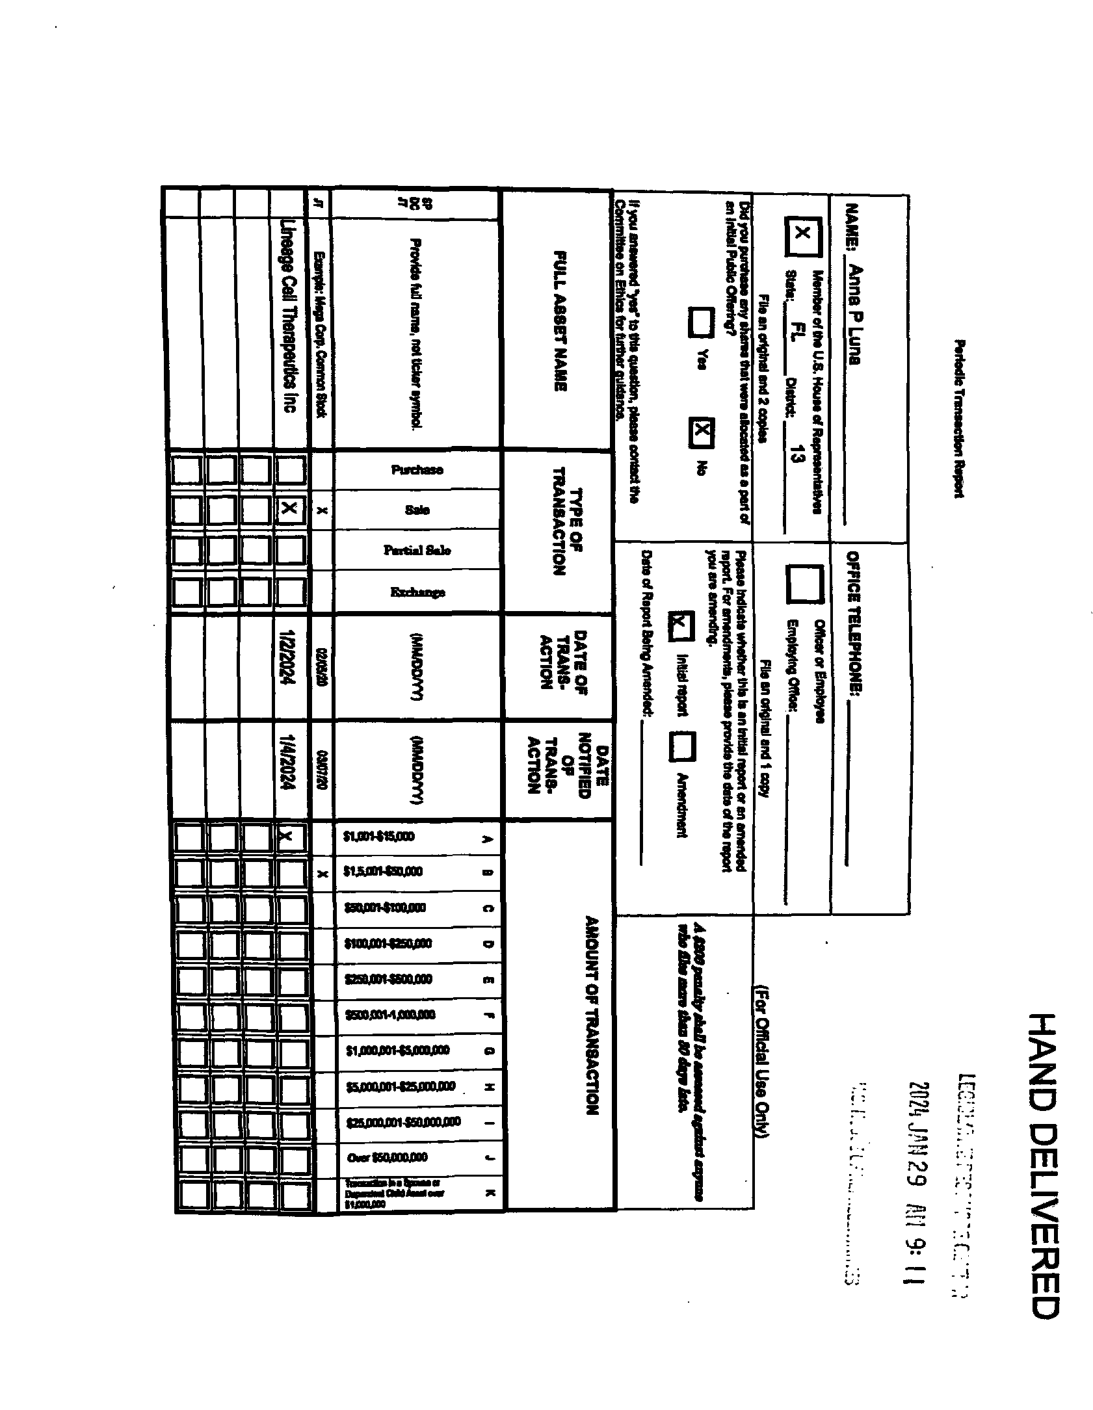
\includegraphics[height=7cm]{sources/house_ocr.png}\\[3pt]
{\footnotesize\textbf{(b) Chambre — OCR.} PDF scanné, ici \emph{couché}~: formulaire à cases, redressé
par deskew avant lecture Vision.}
\end{minipage}

\vspace{12pt}
\begin{minipage}[t]{0.47\textwidth}\centering
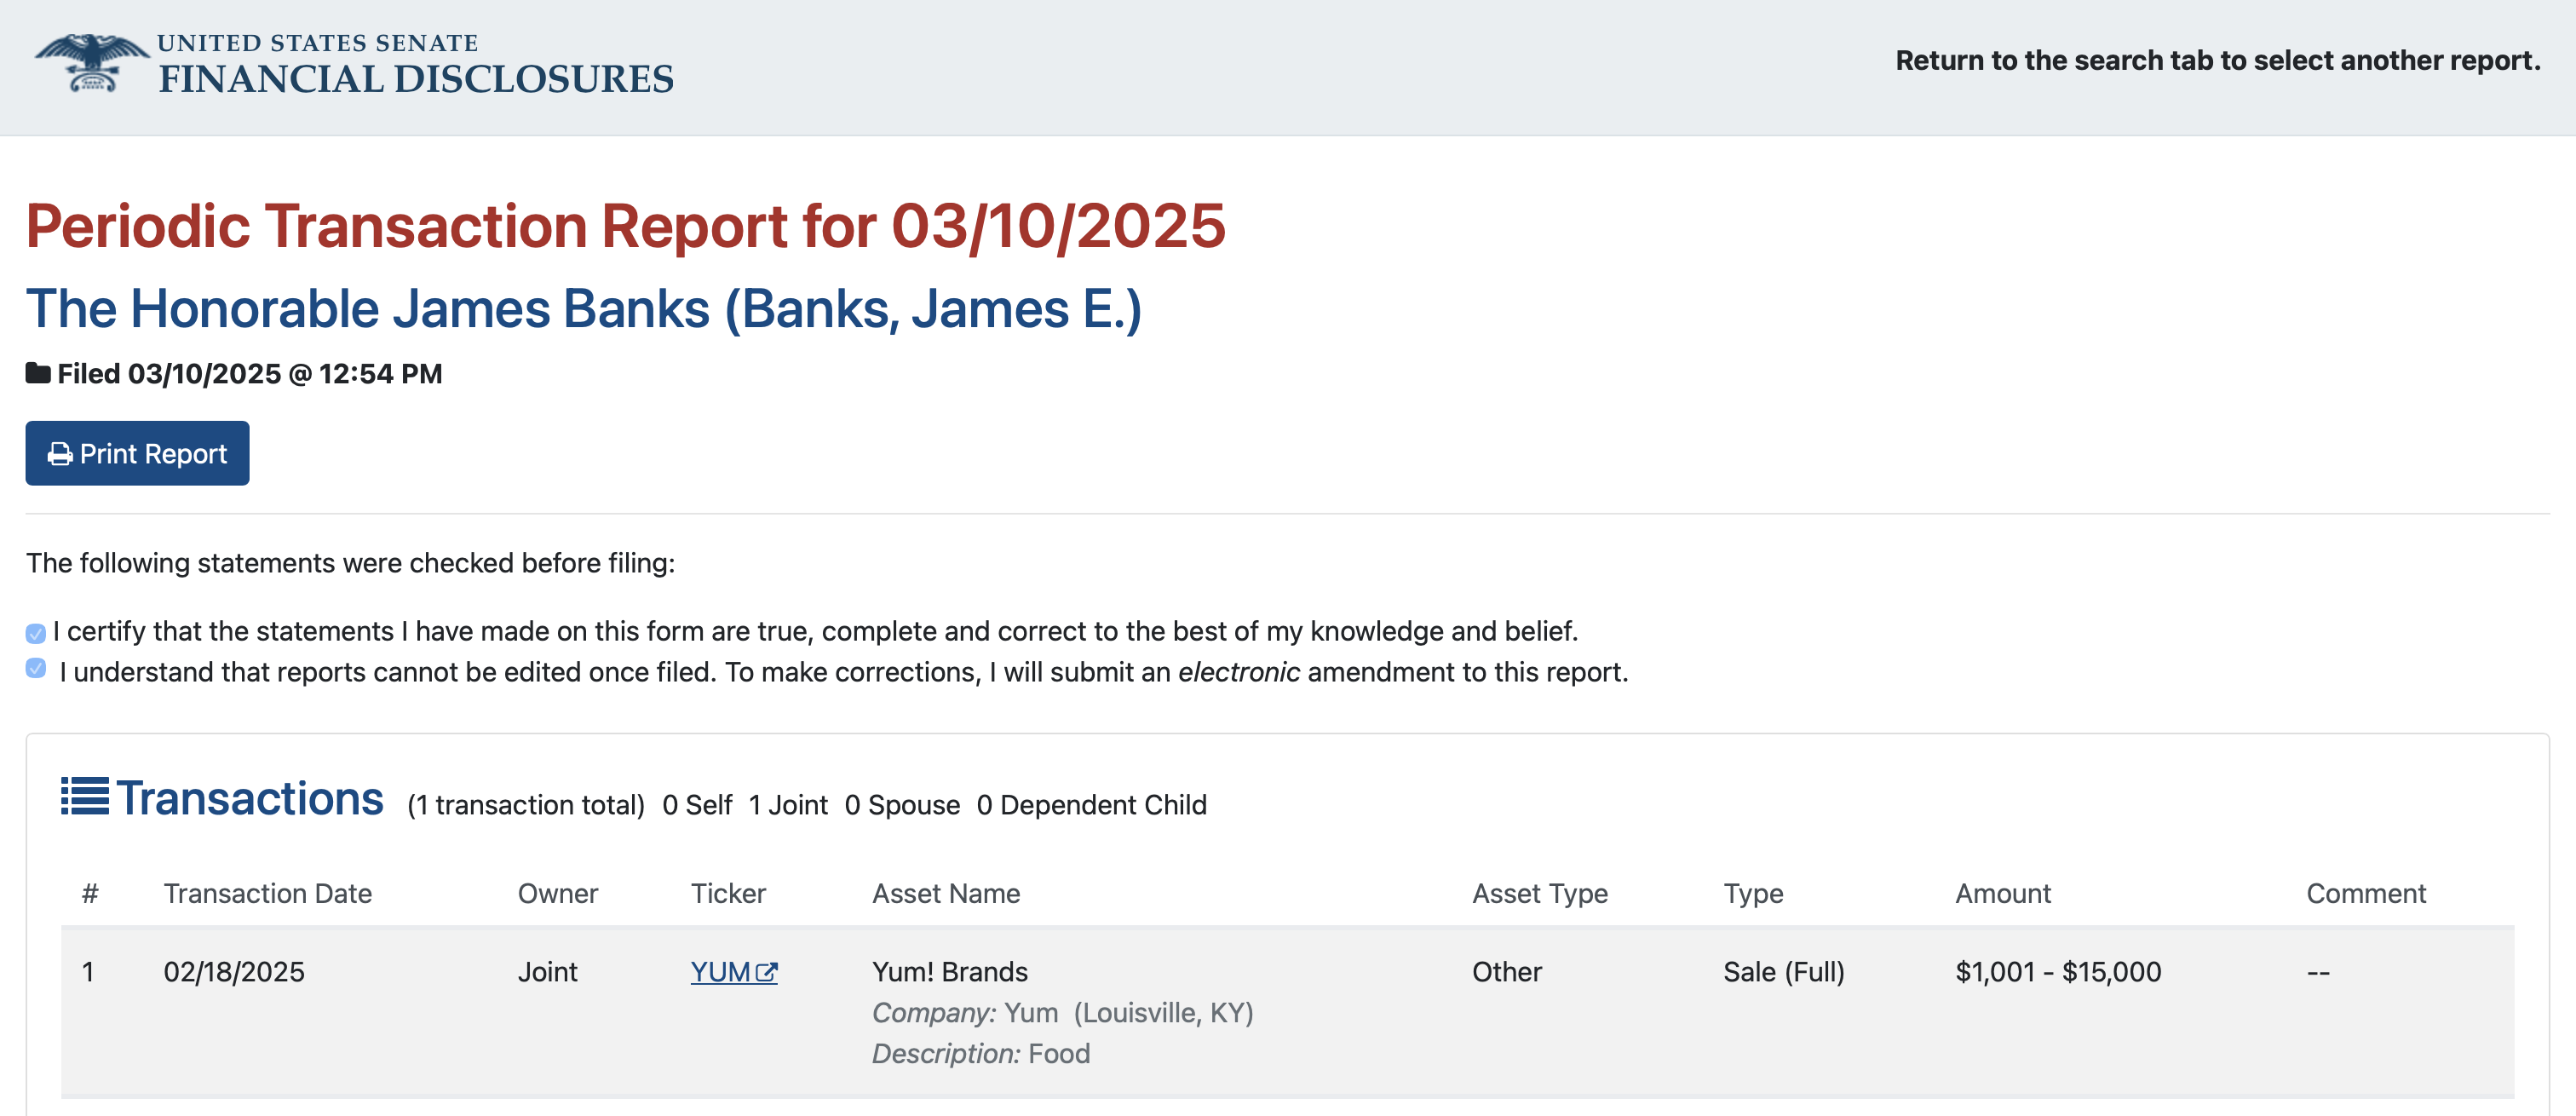
\includegraphics[width=\linewidth]{sources/senate_digital.png}\\[3pt]
{\footnotesize\textbf{(c) Sénat — électronique.} Page web eFD~: ticker cliquable (YUM), type d'opération
et montant — lue par \co{pd.read_html}.}
\end{minipage}\hfill
\begin{minipage}[t]{0.47\textwidth}\centering
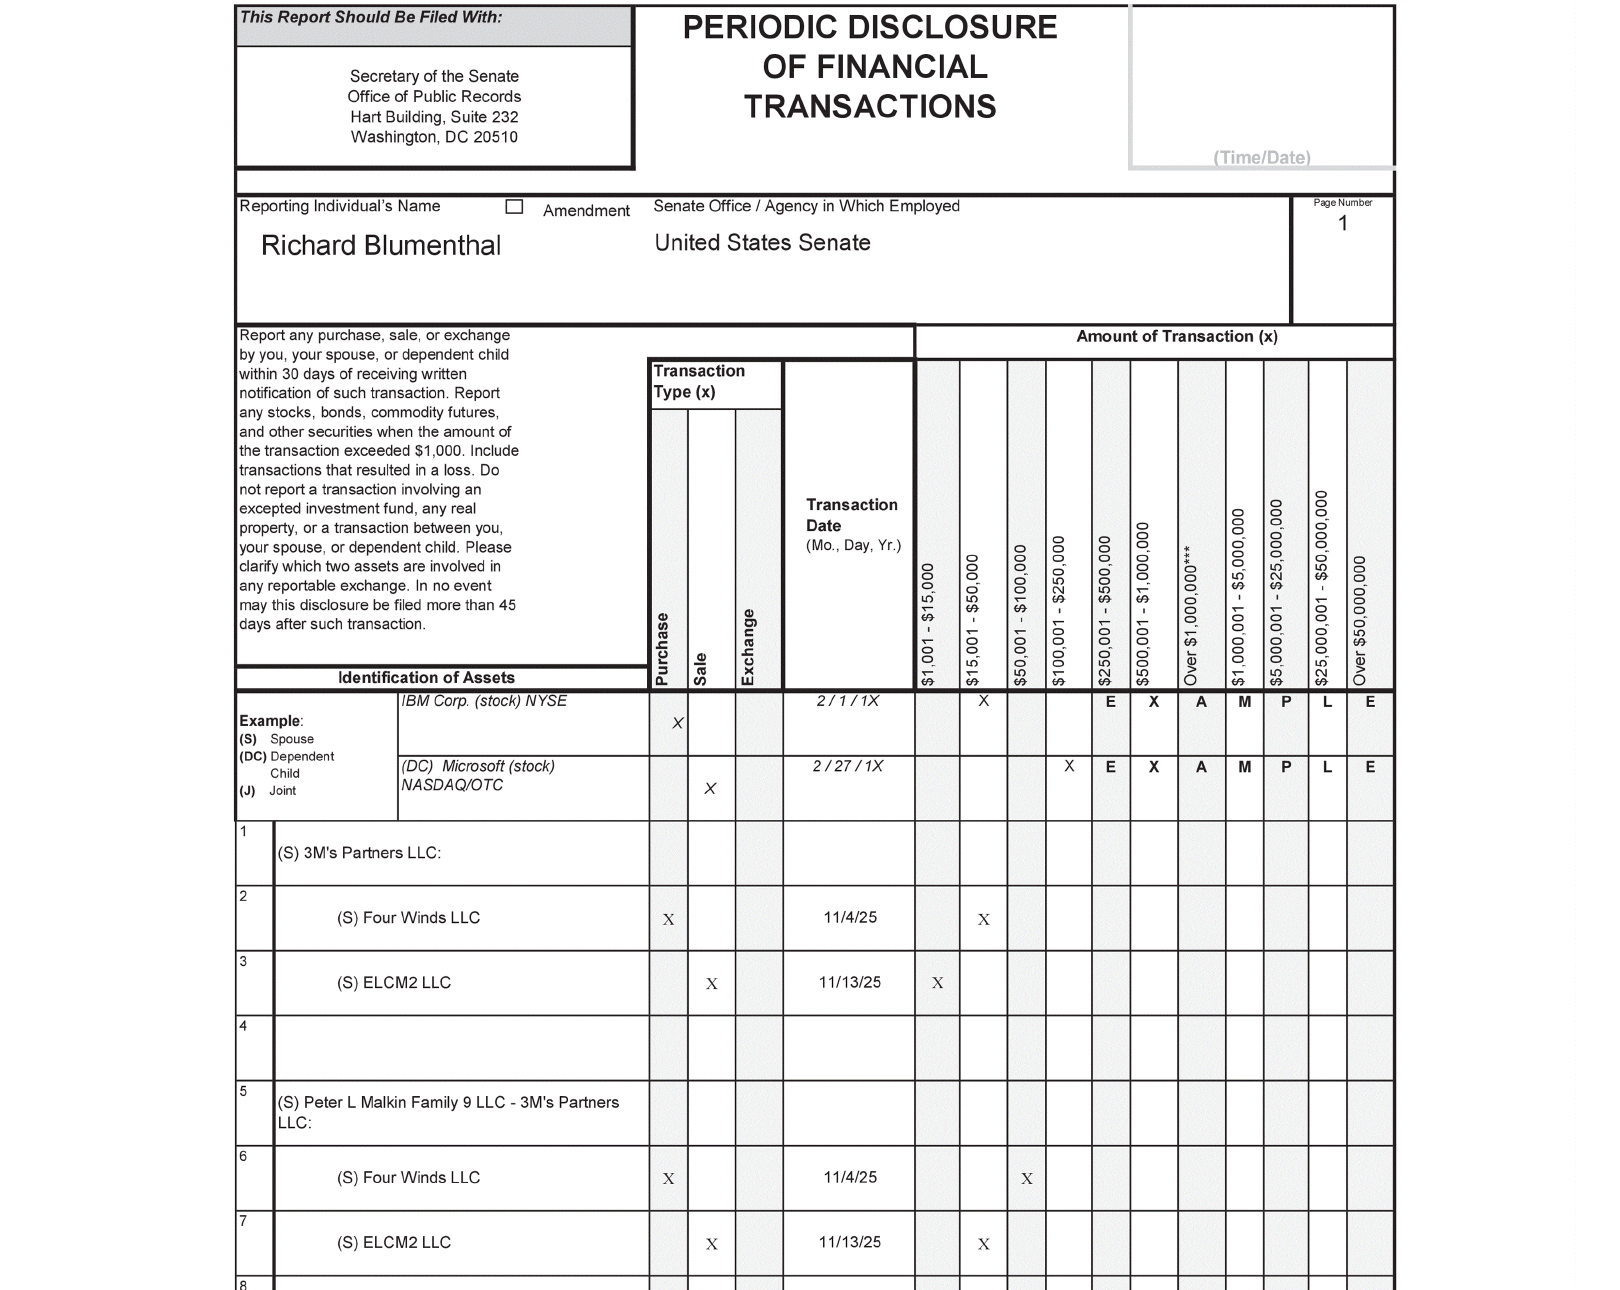
\includegraphics[width=\linewidth]{sources/senate_ocr.png}\\[3pt]
{\footnotesize\textbf{(d) Sénat — OCR.} Formulaire papier scanné (eFD \emph{media})~: lignes à cocher,
fourchettes de montant en colonnes.}
\end{minipage}
\end{center}

\subsection{Annexe B — modules \& fonctions clés}
\label{anx:modules}
Pour chaque module~: son rôle, et ses \textbf{fonctions centrales} (les helpers privés mineurs sont
omis). Le code vit dans \textbf{28 modules} (\co{common/} 11 + \co{house/} 9 + \co{senate/} 8)~;
l'orchestration se lit dans \co{common/pipeline.py:build_steps}, puis \co{house/digital.py:run_year},
\co{house/ocr.py:run_ocr_year}, \co{senate/digital.py:run_year} et \co{senate/fusion.py:main}.
{\footnotesize
\begin{longtable}{>{\ttfamily\footnotesize}p{2.6cm} p{3.9cm} p{8.6cm}}
\toprule
\normalfont\bfseries Module & \bfseries Rôle & \normalfont\bfseries Fonctions clés \\
\midrule\endhead
\multicolumn{3}{l}{\bfseries\color{coreC} common/ — le contrat universel partagé (11)}\\
reference.py & référentiel des élus & \co{load_reference} · \co{Reference} · \co{enrich_identity} · \co{add_years_in_office} · \co{bio_to_committees} \\
schema.py & clé naturelle + dédup & \co{natural_key_hash} (SHA-256 de 7 champs) · \co{add_occurrence_index} · \co{dedup_canonical} (non destructrice) · \co{canonical_ticker} · \co{CORE_FIELDS} \\
sector_enrich.py & secteur GICS → ETF & \co{resolve_yfinance} · \co{resolve_llm} (\co{is_listed}) · \co{enrich_sectors} (+ \co{sector_source}) · \co{GICS_TO_ETF} \\
vision_ocr.py & OCR Vision de référence & \co{detect_rotation} (deskew 4 rotations) · \co{pdf_to_b64_images} · \co{VisionExtractor.prompt_sha} · \co{.extract_cached} \\
crosscheck.py & statut par déposant & \co{per_filer_status} · \co{add_external_counts} · \co{summary} \\
quality.py & rapport qualité (six contrôles) & \co{load_final} · \co{date_coherence} · \co{delay_buckets} · \co{amount_distribution} · \co{coverage_per_member} · \co{backtest_funnel} · \co{build_report} \\
quiver_diagnosis.py & complétude vs Quiver (3 niveaux, \S{}\ref{sec:quiver}) & \co{ticker_inclusion} (N1) · \co{reconcile_dates} (N2, 1-à-1) · \co{field_disagreements} (N3) · \co{build_diagnosis} \\
quiver_scopes.py & validation Quiver multi-scopes & \co{reconcile_scopes} (digital/ocr/both → \co{07c--07f}) · \co{match_breakdown} (par actif \& cluster → \co{07g}/\co{07h}) \\
enrich_tenure.py & ancienneté & \co{add_years_in_office} (append \co{years_in_office} octet-préservant) · \co{main} \\
report_pdf.py & rapport qualité → PDF & \co{md_to_html} · \co{build_pdf} · \co{main} \\
pipeline.py & orchestrateur & \co{build_steps} (séquence en sous-processus) · \co{main} (\co{--years}, \co{--dry-run}) \\
\midrule
\multicolumn{3}{l}{\bfseries\color{houseC} house/ — orchestrateur Chambre (9)}\\
acquire.py & acquisition index + PDF & \co{download_index} · \co{download_pdfs} · \co{main} (\co{--years}) \\
digital.py & PTR électroniques & \co{load_ptr_index} (XML, \co{FilingType=P}) · \co{build_manifest} (tri lisible/non) · \co{parse_ptr} / \co{parse_ptr_legacy} / \co{parse_ptr_dual} · \co{finalize} · \co{run_year} \\
classify_scans.py & classement des scans (A/B/C) & \co{classify_one} (Vision, page 1) · \co{main} \\
ocr.py & scans → FINAL (par an) & \co{run_ocr_year} (Vision + fusion + ticker + secteur + Quiver) · \co{FILERS_C_A_RECUPERER} · \co{DOCS_C_HERITES_2020_2026} (gating manuscrit) \\
identity.py & matcher Chambre & \co{make_matcher} (override→exact+surnoms→nom unique) · \co{_MANUAL_BIO} \\
amounts.py & montant \& opération & \co{amount_midpoint} (milieu de fourchette) · \co{operation_type_from_code} (P/S/E) · \co{HOUSE_OCR_AMOUNT_MAP} \\
tickers.py & ticker + type d'actif & \co{explicit_ticker} · \co{recover_ticker} · \co{infer_asset_type} (par chambre) \\
quiver.py & réconciliation Quiver & \co{reconcile} · \co{norm_ticker} (robuste NaN/vide) \\
echantillon.py & pilote OCR stratifié & \co{run_echantillon} · \co{compare_quiver} \\
\midrule
\multicolumn{3}{l}{\bfseries\color{senateC} senate/ — orchestrateur Sénat (8)}\\
digital.py & eFD électronique & \co{accept_agreement} (CSRF) · \co{fetch_ptr_list} (\co{report_types=[11]}) · \co{fetch_report} · \co{parse_electronic} (\co{pd.read_html}, \co{_find_col}) · \co{run_year} \\
ocr.py & papier \co{.gif} → 06b & \co{discover_index} · \co{ocr_one} (un \co{.gif} → Vision) · \co{build_table} \\
ocr_engine.py & moteur OCR figé & \co{extract_report} · \co{normalize} · \co{_infer_asset_type} \\
fusion.py & fusion + enrich corpus & \co{main} (Étape 1 fusion/an · Étape 2 enrichissement corpus + Quiver) · \co{date_confidence} \\
identity.py & matcher Sénat & \co{load_reference} · \co{make_matcher} (désambiguïsation chambre, exclut délégués) · \co{enrich} \\
ticker.py & ticker 3 voies & \co{resolve_tickers} (explicit→dict→LLM) · \co{llm_resolve_tickers} \\
quiver.py & réconciliation Quiver & \co{reconcile} · \co{norm_ticker} · \co{norm_sense} \\
census_probe.py & census + sondage parser & \co{parse_electronic} · \co{main} \\
\bottomrule
\end{longtable}}
\textit{Les \co{__init__.py} (exports de paquet) et \co{tests/regression/} (golden + reproductions)
complètent le dépôt. Le secteur (\co{common/sector_enrich}) et la clé (\co{common/schema}) sont importés
\emph{en direct} par les deux orchestrateurs — d'où leur place dans \co{common/}.}

\subsection{Annexe C — le schéma FINAL (28 colonnes)}
\label{anx:schema}
{\footnotesize
\begin{longtable}{r >{\ttfamily}p{3.3cm} p{8.2cm} >{\ttfamily\scriptsize}p{3.0cm}}
\toprule
\# & \normalfont\bfseries Colonne & \bfseries Sens & \normalfont\bfseries Remplie par \\
\midrule\endhead
1 & bioguide_id & identifiant officiel du membre & identity \\
2 & declarant_name & nom tel que déposé & parse / OCR \\
3 & chamber & \co{house} / \co{senate} & enrich_identity \\
4 & party & parti & Reference.party \\
5 & state_district & état + district & 03\_ptr\_index \\
6 & committee_membership & commissions (liste) & Reference.committees \\
7 & committees_key_flag & commission « clé » ? & reference \\
8 & transaction_date & date de la transaction & parse / OCR \\
9 & disclosure_date & date de divulgation (dépôt) & 03\_ptr\_index / eFD \\
10 & ticker & symbole boursier & tickers / ticker \\
11 & asset_description & libellé de l'actif & parse / OCR \\
12 & asset_type & type d'actif & infer_asset_type \\
13 & sector_gics & secteur GICS & sector_enrich \\
14 & etf_proxy & ETF SPDR du secteur & GICS\_TO\_ETF \\
15 & operation_type & Purchase / Sale / … & operation_type_from_code \\
16 & amount_range & fourchette déclarée & parse / OCR \\
17 & amount_midpoint & milieu de la fourchette & amount_midpoint \\
18 & amount_split_flag & lot multi-actifs ? & parse \\
19 & owner & propriétaire (self/spouse…) & parse / OCR \\
20 & doc_id & identifiant du PTR & 03\_ptr\_index \\
21 & source_url & URL de la source & 03\_ptr\_index \\
22 & natural_key_hash & clé de dédup (7 champs) & schema \\
23 & occurrence_index & rang du lot intra-dépôt & add_occurrence_index \\
24 & provenance & \co{*-electronic} / \co{*-ocr} & pipeline \\
25 & date_confidence & plausible / implausible (75 j) & date_confidence \\
26 & ticker_source & explicit / elec\_dict / llm / none & tickers / ticker \\
27 & sector_source & yfinance / llm / manual / none & sector_enrich \\
28 & years_in_office & ancienneté à la date du trade & enrich_tenure \\
\bottomrule
\end{longtable}}
\textit{L'ordre exact diffère légèrement entre Chambre et Sénat (\co{date_confidence} plus tôt au
Sénat)~; le contenu garanti — les 12 champs « métier » — est identique. Les 27 colonnes d'assemblage
(\co{HOUSE_FINAL_SCHEMA} / \co{SENATE_FINAL_SCHEMA}) + \co{years_in_office} = 28. Le dictionnaire de la
\textbf{table de recherche canonique} (36 colonnes) est au \S{}\ref{sec:nettoyage}.}

\subsection{Annexe D — métriques vérifiées (recalculées depuis les FINAL)}
\label{anx:metrics}
\textbf{Lue après le rapport, cette annexe dit si l'extraction a bien marché.} Chaque tableau indique sa
\textbf{source}~: \textbf{[A]} chiffre \emph{asserté} par le filet de non-régression
\co{tests/regression/audit_metrics.py} (un écart le fait échouer)~; \textbf{[Q]} recalculé par
\co{common/quality.py} (descriptif)~; \textbf{[D]} recalculé par \co{common/quiver_diagnosis.py}
(diagnostic Quiver, offline déterministe). La version exhaustive — toutes les années, tous les champs —
est le rapport qualité \co{docs/RAPPORT_QUALITE.md}, dont cette annexe ne retient que l'essentiel.

\textbf{D.1 — Volumes par an \& identité} \hfill {\footnotesize\textbf{[A]} totaux \& identité · \textbf{[Q]} ventilation par an}
\begin{center}\small
\begin{tabular}{l rrrr @{\hspace{1.4em}} rrrr}
\toprule
& \multicolumn{4}{c}{\bfseries\color{houseC}Chambre} & \multicolumn{4}{c}{\bfseries\color{senateC}Sénat}\\
\cmidrule(lr){2-5}\cmidrule(lr){6-9}
\bfseries An & élec. & OCR & FINAL & dépos. & élec. & OCR & FINAL & dépos.\\
\midrule
2014 & 2\,340 & 8\,389 & 10\,729 & 101 & 651 & 241 & 892 & 19 \\
2015 & 4\,791 & 4\,789 & 9\,580 & 101 & 1\,151 & 281 & 1\,432 & 27 \\
2016 & 4\,655 & 2\,907 & 7\,562 & 107 & 995 & 427 & 1\,422 & 30 \\
2017 & 4\,546 & 8\,036 & 12\,582 & 112 & 1\,320 & 210 & 1\,530 & 33 \\
2018 & 4\,437 & 10\,190 & 14\,627 & 97 & 1\,236 & 641 & 1\,877 & 31 \\
2019 & 5\,188 & 7\,366 & 12\,554 & 104 & 1\,158 & 506 & 1\,664 & 35 \\
2020 & 6\,885 & 9\,207 & 16\,092 & 111 & 1\,655 & 255 & 1\,910 & 33 \\
2021 & 5\,454 & 6\,936 & 12\,390 & 121 & 632 & 281 & 913 & 35 \\
2022 & 3\,601 & 11\,857 & 15\,458 & 112 & 912 & 182 & 1\,094 & 27 \\
2023 & 4\,168 & 6\,687 & 10\,855 & 100 & 1\,032 & 97 & 1\,129 & 30 \\
2024 & 2\,701 & 6\,948 & 9\,649 & 98 & 946 & 84 & 1\,030 & 24 \\
2025 & 7\,576 & 6\,159 & 13\,735 & 107 & 859 & 477 & 1\,336 & 31 \\
2026 & 2\,386 & 3\,790 & 6\,176 & 85 & 479 & 303 & 782 & 22 \\
\midrule
\bfseries Tot. & \bfseries 58\,728 & \bfseries 93\,261 & \bfseries 151\,989 & \bfseries 367$^\ast$ & \bfseries 13\,026 & \bfseries 3\,985 & \bfseries 17\,011 & \bfseries 78$^\ast$\\
\bottomrule
\end{tabular}
\end{center}
{\footnotesize \emph{élec.} = électronique~; \emph{dépos.} = \co{bioguide_id} \emph{uniques} sur 13 ans
($^\ast$~total~; la colonne annuelle recompte un élu chaque année). Le tableau compte les
\textbf{transactions uniques} par année de dépôt (\co{file_year})~; le brut fait \textbf{170\,920} lignes
(Chambre 152\,081 + Sénat 18\,839), ramenées à \textbf{169\,000} par la dédup cross-année (1\,920
re-divulgations). \textbf{Assertés [A]}~: les totaux, l'identité (\textbf{367} bioguides Chambre,
\textbf{78} Sénat~; \textbf{0} ligne sans bioguide) et le golden octet-à-octet (\textbf{230} fichiers
Chambre, \textbf{138} Sénat).}

\textbf{D.2 — Couverture \& qualité, par sous-corpus} \hfill {\footnotesize\textbf{[Q]}}
\begin{center}\footnotesize
\begin{tabular}{l r rrr r r}
\toprule
\bfseries Sous-corpus & \bfseries n & \bfseries ticker\,\% & \bfseries secteur\,\% & \bfseries commissions\,\% & \bfseries dates cohér.\,\% & \bfseries montant\,\%\\
\midrule
{\color{houseC}Chambre électronique} & 58\,728 & 83,8 & 77,7 & 54,8 & 99,9 & 100,0 \\
{\color{houseC}Chambre OCR} & 93\,261 & 84,3 & 81,1 & 80,8 & 99,8 & 98,9 \\
{\color{senateC}Sénat électronique} & 13\,026 & 84,1 & 77,8 & 53,0 & 99,9 & 100,0 \\
{\color{senateC}Sénat OCR} & 3\,985 & 57,4 & 46,2 & 64,9 & 98,8 & 99,4 \\
\bottomrule
\end{tabular}
\end{center}
{\footnotesize \emph{dates cohér.\,\%} = part où la divulgation suit la transaction (\co{disclosure ≥
transaction}, parmi les dates exploitables)~; \emph{montant\,\%} = montant renseigné. Identité = 100\,\%
partout, ancienneté 99,9--100\,\%. Les \textbf{six contrôles globaux} (\S{}\ref{sec:qualite}) en bref~: délai
médian \textbf{27~j} Chambre / \textbf{24~j} Sénat (≤45~j~: 87,3 / 86,9\,\%)~; montant médian
\textbf{8\,000\,\$} (quartile haut 32\,500\,\$, moyenne 58\,314\,\$)~; \textbf{445} déposants, dont
\textbf{294} à ≥10 transactions et \textbf{236} sur ≥3 ans~; achats revendus sous 12 mois 67,7 / 48,3\,\%.
Détail \textbf{par année} dans \co{RAPPORT_QUALITE.md}.}

\textbf{D.3 — Composition des transactions, par sous-corpus} \hfill {\footnotesize\textbf{[Q]} (\% du corpus)}
\begin{center}\small
\begin{tabular}{l rr @{\hspace{1.4em}} rrrr}
\toprule
& \multicolumn{2}{c}{\bfseries opération} & \multicolumn{4}{c}{\bfseries détenteur du compte}\\
\cmidrule(lr){2-3}\cmidrule(lr){4-7}
\bfseries Sous-corpus & achat & vente & soi-même & conjoint & joint & enfant\\
\midrule
Chambre électronique & 50,4 & 48,6 & 49,3 & 20,4 & 26,7 & 3,6 \\
Chambre OCR & 52,2 & 47,3 & 10,3 & 47,9 & 13,6 & 28,2 \\
Sénat électronique & 50,2 & 48,8 & 16,8 & 38,7 & 42,1 & 2,4 \\
Sénat OCR & 56,4 & 43,0 & 48,8 & 49,5 & 1,5 & 0,3 \\
\bottomrule
\end{tabular}
\end{center}
\begin{center}\small
\begin{tabular}{l rrrrrrrr}
\toprule
\bfseries Type d'actif (\%) & action & option & oblig. État & munis & oblig. corp. & fonds & autre & manquant\\
\midrule
Chambre électronique & 58,5 & 1,2 & 4,1 & 0,0 & 0,0 & 0,0 & 4,9 & 31,3 \\
Chambre OCR & 79,2 & 0,0 & 0,8 & 0,0 & 0,4 & 3,2 & 0,3 & 16,2 \\
Sénat électronique & 73,0 & 4,7 & 0,0 & 7,7 & 3,0 & 0,0 & 6,5 & 5,1 \\
Sénat OCR & 40,4 & 0,0 & 0,0 & 0,7 & 2,2 & 0,0 & 41,2 & 15,5 \\
\bottomrule
\end{tabular}
\end{center}
{\footnotesize « munis » = obligations municipales~; « autre » et « manquant » = actifs non cotés ou non
identifiés (une bonne part des « manquants » à ticker valide est récupérée \emph{ticker d'abord} par la
table de recherche, \S{}\ref{sec:nettoyage}). Le Sénat OCR ($\approx$57\,\% de non-coté ou non identifié) est
ce qui le met hors de portée de Quiver (\S{}\ref{sec:quiver}).}

\textbf{D.4 — Validation Quiver~: corroboration par année et par cluster} \hfill {\footnotesize\textbf{[D]}}
\begin{center}\small
\begin{tabular}{l rrr @{\hspace{2.6em}} l rrr}
\toprule
\bfseries An & corrob. & only-nous & \bfseries \% & \bfseries An & corrob. & only-nous & \bfseries \% \\
\midrule
2014 & 1\,930 & 3\,984 & 32,6 & 2021 & 6\,945 & 2\,803 & 71,2 \\
2015 & 540 & 2\,711 & 16,6 & 2022 & 11\,011 & 1\,286 & 89,5 \\
2016 & 291 & 1\,458 & 16,6 & 2023 & 7\,522 & 442 & 94,5 \\
2017 & 3\,729 & 2\,241 & 62,5 & 2024 & 6\,797 & 481 & 93,4 \\
2018 & 7\,243 & 2\,722 & 72,7 & 2025 & 11\,095 & 408 & 96,5 \\
2019 & 7\,630 & 1\,899 & 80,1 & 2026 & 4\,740 & 348 & 93,2 \\
2020 & 10\,025 & 2\,801 & 78,2 & & & & \\
\bottomrule
\end{tabular}
\end{center}
{\footnotesize Corroboration au niveau \textbf{action} (Chambre, \co{asset_type=Stock})~: \emph{corrob.} =
actions appariées à Quiver (exact + date proche)~; \emph{only-nous} = actions réelles qu'on a et que Quiver
n'a pas (non corroborables)~; \% = corrob. / (corrob. + only-nous). Agrégé~: \textbf{87,2\,\%} sur
2020--2026, \textbf{58,7\,\%} sur 2014--2019 — Quiver est mince avant $\approx$\,2017 (\S{}\ref{sec:quiver}).}

\begin{center}\small
\begin{tabular}{l rr rrr}
\toprule
\bfseries Cluster (Chambre OCR) & n lignes & n docs & date plaus.\,\% & ticker\,\% & Quiver a le trade\,\%\\
\midrule
A — tapé droit & 5\,956 & 59 & 99,6 & 84,5 & \textbf{88,0} \\
B — tapé couché & 84\,787 & 1\,517 & 96,4 & 84,3 & \textbf{65,2} \\
C — manuscrit (conservé) & 2\,518 & 193 & 98,6 & 83,3 & \textbf{12,9} \\
\bottomrule
\end{tabular}
\end{center}
{\footnotesize \emph{date plaus.\,\%} / \emph{ticker\,\%} = qualité interne (sans Quiver)~; \emph{Quiver a
le trade\,\%} = part de nos trades cotés que Quiver possède aussi (membre + ticker + sens, avec ou sans
date). Sur le manuscrit (C), la qualité interne reste haute mais la corroboration s'effondre~: faute de
pouvoir le confirmer contre la vérité-terrain, il est écarté par défaut — politique rejouable, exceptions
explicites (\S{}\ref{sec:hocr}).}

\textbf{D.5 — Concentration de l'activité} \hfill {\footnotesize\textbf{[Q]}}
\begin{center}\small
\begin{tabular}{l r rr r}
\toprule
\bfseries Sous-corpus & \bfseries n déposants & \bfseries HHI & \bfseries Gini & \bfseries top-10 du volume\,\%\\
\midrule
{\color{houseC}Chambre électronique} & 309 & 432,4 & 0,873 & 57,6 \\
{\color{houseC}Chambre OCR} & 125 & 2\,561,1 & 0,953 & 94,7 \\
{\color{senateC}Sénat électronique} & 75 & 943,7 & 0,826 & 79,5 \\
{\color{senateC}Sénat OCR} & 14 & 2\,671,5 & 0,753 & 100,0 \\
\bottomrule
\end{tabular}
\end{center}
{\footnotesize \emph{HHI} (indice de Herfindahl, $\in [0,\,10\,000]$) et \emph{Gini} ($\in [0,\,1]$) mesurent
la concentration du volume entre déposants~: 0 = parts égales, maximum = un seul capte tout.
Déposants-papier dominants~: Khanna \textbf{41\,080} transactions (44,0\,\% de l'OCR Chambre), McCaul
27\,123, Harshbarger 3\,665~; au Sénat, Blumenthal 1\,543 (38,7\,\% du papier). Top tickers par volume
estimé~: MSFT 550,1~M\$, AAPL 120,4, FDX 119,9.}

\subsection{Annexe E — reproduire / lancer}
\label{anx:run}
{\footnotesize
\begin{verbatim}
# Installation
python3.12 -m venv .venv && ./.venv/bin/pip install -e .

# Pipeline complet (reseau + API Vision requis) ; --dry-run = voir la sequence
./.venv/bin/python -m common.pipeline --years 2014-2026
./.venv/bin/python -m common.pipeline --years 2014-2019 --acquire   # re-telecharge index + PDF
./.venv/bin/python -m common.pipeline --years 2024 --dry-run

# Rapport de qualite (offline, lecture seule des FINAL)
#   -> docs/RAPPORT_QUALITE.md + docs/quality/*.png
./.venv/bin/python -m common.quality

# Table de recherche canonique (offline, depuis les FINAL)
#   -> data/clean/transactions_backtest_2014_2026.csv (134 464 x 36)
#   notebook : Nettoyage_Backtest_2014_2026.ipynb (executer toutes les cellules)

# Filet "zero changement" (doit afficher ZERO ECART)
./.venv/bin/python tests/regression/check_golden.py         # Chambre, 230
./.venv/bin/python tests/regression/senate_check_golden.py  # Senat,   138
./.venv/bin/python tests/regression/test_senate_repro.py    # reproductions
\end{verbatim}}

\vfill
\begin{center}\footnotesize\itshape
Document dérivé et vérifié sur le code source réel, les tables FINAL et la table de recherche canonique du
dépôt. Toute divergence avec une autre documentation doit être tranchée en faveur du code et des données.
Quiver = vérification externe, jamais réinjecté.
\end{center}

\end{document}
